%%%%%%%%%%%%%%%%%%%%%%%%%%%%%%%%%%%%%%%%%%%%%%%%%%%%%%%%%%%%%%%%%%%%%%%%%%%%%%%%%%%%%%%%%%%%%
%% TC-ViTok — BMVC 2026 submission (anonymous, double-blind).
%%
%% This file currently uses the ICML 2021 template as a stand-in. To switch to
%% the official BMVC 2026 template:
%%   1. Download bmvc2k.cls (or whatever 2026 ships) from
%%      https://bmvc2026.bmva.org/calls/call-for-papers/
%%   2. Replace lines 6-38 below with:
%%        \documentclass{bmvc2k}
%%        \usepackage{...}   % the same packages you see below
%%   3. Wrap the \icmltitle / \icmlauthorlist block with the BMVC equivalent
%%      (\title{...} \addauthor{}{}{}{} ... \runninghead{}{}).
%%   4. Comment out \usepackage[accepted]{icml2021} and \icmltitlerunning{...}.
%%
%% IMPORTANT: BMVC 2026 is double-blind. Author names, affiliations, the GitHub
%% URL, and any internal acknowledgments are commented out below. Verify before
%% submission that no identifying information leaks via figures or supplementary
%% material.
%%%%%%%%%%%%%%%%%%%%%%%%%%%%%%%%%%%%%%%%%%%%%%%%%%%%%%%%%%%%%%%%%%%%%%%%%%%%%%%%%%%%%%%%%%%%%

\documentclass{article}

% Input encoding (em-dashes, smart quotes etc compile cleanly in pdflatex).
\usepackage[utf8]{inputenc}
\usepackage[T1]{fontenc}

\usepackage{microtype}
\usepackage{graphicx}
\usepackage{subfigure}
\usepackage{booktabs}
\usepackage{hyperref}
\usepackage{amsmath}
\usepackage{amssymb}
\usepackage{xcolor}
\usepackage{tikz}
\usetikzlibrary{arrows.meta,positioning,shapes.geometric,fit,calc,backgrounds,decorations.pathreplacing,decorations.markings,patterns,shadings,shadows}

% --- Professional color palette (used by custom diagrams) ---
\definecolor{tcblue}{RGB}{45,95,165}
\definecolor{tcbluelight}{RGB}{210,225,245}
\definecolor{tcaccent}{RGB}{198,69,53}
\definecolor{tcaccentlight}{RGB}{250,225,220}
\definecolor{tcgreen}{RGB}{60,135,90}
\definecolor{tcgreenlight}{RGB}{220,238,225}
\definecolor{tcgold}{RGB}{205,150,40}
\definecolor{tcgoldlight}{RGB}{250,238,205}
\definecolor{tcgray}{RGB}{96,108,124}
\definecolor{tcgraylight}{RGB}{235,238,243}
\definecolor{tcink}{RGB}{32,40,52}
\definecolor{tcpaper}{RGB}{252,252,250}
\usepackage{pgfplots}
\pgfplotsset{compat=1.18}
\usepackage{pifont}

\newcommand{\theHalgorithm}{\arabic{algorithm}}

\usepackage[accepted]{icml2021}

% Running title — prevents "Title suppressed due to excessive length" in page headers
\icmltitlerunning{TC-ViTok: Failure-Mode Taxonomy for Pre-LLM Token Compression}

% -------------------------------------------------------------------
% Convenience macros
\newcommand{\vcoarse}{\mathbf{v}_{c}}
\newcommand{\vfine}{\mathbf{v}_{f}}
\newcommand{\qemb}{\mathbf{q}}
\newcommand{\sN}{\mathbf{s}_N}
\newcommand{\vsel}{\mathbf{v}_{sel}}
\newcommand{\vunsel}{\mathbf{v}_{unsel}}
\newcommand{\vmerged}{\mathbf{v}_{merged}}
\newcommand{\bsig}{\boldsymbol{\sigma}}
% -------------------------------------------------------------------

\begin{document}

\twocolumn[
\icmltitle{TC-ViTok: A Failure-Mode Taxonomy for Pre-LLM Visual Token\\
           Compression, with a Parameter-Free Recipe}

% Anonymous for double-blind review.
\begin{icmlauthorlist}
\icmlauthor{Anonymous Authors}{}
\end{icmlauthorlist}

\icmlkeywords{Vision-Language Models, Visual Token Compression, Query-Conditioned Selection,
              Straight-Through Estimator, Co-Adaptation, BMVC 2026 Submission}

\vskip 0.3in
]

% ===================================================================
\begin{abstract}
We report a trained, pre-LLM, query-conditioned visual-token selector
(TC-ViTok) at LLaVA-1.5-7B scale with a matched same-LoRA, same-SFT,
full-576-token reference (\textsc{LoRA-576}). At $4{\times}$ compression
(measured as the $k{=}144$ selected-token ratio), TC-ViTok incurs a measured
cost of $-4.1$ VQAv2, $-3.4$ GQA, and $-7.4$ POPE points --- a cost we report
rather than hide.

Two empirical observations follow from this comparison. First, the converged
selector is empirically close to query-agnostic: zeroing the CLIP query
embedding at inference produces equal or marginally better accuracy, indicating
that the architecture's query-routing channel is not used strongly at this
scale. Second, the converged selector exhibits a structured per-position prior
with a localized region whose inference-time masking improves exact-match
VQA-score by $+2.2$ pp on Final, ranks at the 90th percentile of 10
size-matched random-rectangle controls ($p{=}0.0107$, one-tailed sign test).
The effect is positive on two related checkpoints but reverses sign on an
independently retrained seed, so we treat it as a low-utility-allocation
diagnostic rather than a checkpoint-invariant mechanism.

To explain why compression does not close the \textsc{LoRA-576} gap, we
document three training-dynamics pathologies we encountered while training a
query-conditioned visual-token selector co-optimized with LLM adapters before
the LLM. We present them as concrete, testable hypotheses about pre-LLM
trainable compression more broadly; their universality is an open question we
explicitly invite future work to resolve. \emph{Co-adaptation oscillation}
produces limit cycles whose period grew from approximately 5K to 15K steps as
the selector learning rate dropped $25{\times}$ across the two finite-period
measurements available (the frozen-pooler control has no cycle). We report this
as a qualitative trend, not a scaling law; two data points are insufficient to
fit a functional form. \emph{BudgetPredictor
collapse} sends per-sample token budgets to $k_{\max}$ whenever
$\lambda_b\!\leq\!0.05$, with a narrow stable window of $[0.08, 0.15]$.
\emph{Warm-start dependence} prevents from-scratch convergence at LLaVA-1.5
scale across two selector variants and three LoRA capacities. We sidestep each
pathology with a parameter-free token merge, a calibrated $\lambda_b$, and a
staged curriculum on a converged base.
\end{abstract}

% ===================================================================
\section{Introduction}
\label{sec:intro}

Pre-LLM visual token compression — reducing the visual sequence before it enters the
LLM, saving all prefill FLOPs — does not naively converge when the selector is
co-trained with LLM adapters. This paper is about why, and what to do about it.

Modern VLMs such as LLaVA-1.5~\cite{liu2024llava} attach a large language model (LLM)
to a frozen CLIP ViT-L/14 vision encoder. At inference, the encoder maps a
$336\times336$ image to $576$ patch tokens ($24\times24$ grid), which are prepended to
the tokenized question and fed into the LLM. Since attention cost is quadratic in
sequence length, these 576 visual tokens dominate prefill FLOPs — and the budget is
determined by image resolution, not by what the question requires.

Prior work compresses tokens either query-agnostically (ToMe~\cite{bolya2022token},
EViT~\cite{liang2022evit}, FastV~\cite{chen2024fastv},
PruMerge~\cite{shang2024llava}) or inside the LLM's attention layers, after all tokens
have been injected (SparseVLM~\cite{zhang2025sparsevlm},
FocusLLaVA~\cite{zhu2024focusllava}). Pre-LLM compression with a learned
query-conditioned selector is the architecturally natural design: it saves LLM FLOPs
and is modular. It also does not converge in the obvious training setup.

We attempted this design and found that the obvious joint training procedure fails in
three coupled ways: co-adaptation oscillation, budget-head collapse, and warm-start
dependence. We characterize each failure quantitatively, derive an architectural recipe
that sidesteps two of them by construction and characterizes the third empirically, and
report an honest compression cost against the matched same-LoRA baseline
(\textsc{LoRA-576}). TC-ViTok's role in the paper is to make these
failure modes observable under a realistic LLaVA-scale training setup.

We emphasize that TC-ViTok loses to a matched LoRA-576 no-compression
reference by 4.1 / 3.4 / 7.4 points on VQAv2 / GQA / POPE. The paper's
contribution is the characterization of why pre-LLM trainable compression
fails to close this gap, not the method that fails to.

Practically, the paper is most useful as a map. If future work attempts
trainable pre-LLM token compression at LLaVA-1.5-7B scale, our results suggest
it should budget for co-adaptation oscillation, budget-head collapse, and
warm-start dependence, and should test whether the converged selector is
actually using the query signal rather than assuming architectural
query-conditioning is realized by training.

We make three contributions.

\textbf{(1)~A failure-mode taxonomy for pre-LLM trainable token compression.}
Three coupled pathologies arise in our setting when a learnable selector is jointly trained with
LLM adapters: (a)~\emph{GAN-style co-adaptation oscillation} whose period
increases as selector learning rate decreases in the measured trainable-pooler
family; (b)~\emph{BudgetPredictor collapse}
to $k{=}k_{\max}$ whenever $\lambda_b\!\leq\!0.05$; and (c)~\emph{warm-start
dependence} — from-scratch attempts plateau $2$--$10{\times}$ above the warm-started
ceiling regardless of TPN variant (Section~\ref{sec:warmstart},
Table~\ref{tab:warmstart}).
All evidence for this taxonomy comes from one codebase and one
(encoder, LLM, selector) triple; we present the taxonomy as a set of
portable hypotheses, not as a universality theorem.

\textbf{(2)~An architectural recipe that sidesteps two failures and characterizes
the third.}
(i)~A tau-independent additive STE correction (Eq.~\ref{eq:taufix}) that keeps
TPN-score gradients non-zero at any annealed temperature; (ii)~\emph{Informative
Token Merge}, parameter-free by design, which eliminates the co-adaptation loop by
construction — removing the trainable bridge removes the closed gradient circuit;
and (iii)~a \emph{TPN warmup $\to$ joint warm-freeze $\to$ adaptive budget}
curriculum whose stage ordering is the only ordering of TPN-warmup, joint-freeze,
and adaptive-budget stages we tested that achieves convergence; exhaustive
testing of alternative orderings is left to future work. The warm-start
dependence (FM3) is characterized
empirically but not defeated: from-scratch training does not converge at this scale
regardless of architecture or curriculum order.

\textbf{(3a)~Empirical query-agnostic convergence at LLaVA-7B scale.}
The trained query-conditioned TPN, evaluated on three benchmarks at
$k{=}144$, produces equal or marginally better accuracy when the CLIP query
embedding is zeroed at inference (E3, \S\ref{sec:limits} L7; $+0.40$ /
$+0.33$ / $+0.28$ pp on VQAv2 / GQA / POPE). On Adaptive v2, the same
5K-sample protocol gives $+0.56$ / $-0.16$ / $+0.41$ pp, so zeroing the query
again produces no material degradation. This is an unexpected property of joint
optimization at this scale, and to our knowledge has not been reported in prior
pre-LLM compression work.

\textbf{(3b)~Structured per-position prior with a localized low-utility
region.}
The converged selector exhibits strong per-position selection-frequency
heterogeneity (Fig.~\ref{fig:positional-prior}) and a localized region whose
inference-time masking improves accuracy at the 90th percentile of random
controls (M1--M3, \S\ref{sec:limits} L9). The direction is positive on Final,
Adaptive v2, and v3, but negative on an independently retrained seed-7
checkpoint; this makes L9 an observational low-utility-allocation finding
rather than a claim of checkpoint-invariant dead-zone causality.

% ===================================================================
\section{Related Work}
\label{sec:related}

\textbf{Query-agnostic visual token compression.}
ToMe~\cite{bolya2022token} merges visually similar tokens via bipartite matching inside
ViT layers, achieving 2$\times$ throughput at modest accuracy loss on classification.
DynamicViT~\cite{rao2021dynamicvit} learns binary dropping masks at intermediate layers
via Gumbel-Softmax, trained with distillation.
EViT~\cite{liang2022evit} uses CLS-token attention to rank tokens and fuses low-importance
ones.
Post-encoder methods include LLaVA-PruMerge~\cite{shang2024llava}, which prunes by
CLS-attention rank then merges pruned tokens with nearest retained neighbors via
key-similarity weighting.
FastV~\cite{chen2024fastv} observes that LLM text-to-visual attention collapses after
layer 2 and prunes low-attention tokens at that boundary.
All these methods share a fundamental limitation: the compression decision is made
without knowledge of the query, systematically harming spatially-grounded tasks
(localization, OCR) more than global tasks~\cite{chen2024fastv, endo2025feather}.

\textbf{Query-aware compression.}
BLIP-2~\cite{li2023blip2}'s Q-Former extracts visual tokens via cross-attention with
learned query embeddings, but the queries are fixed parameters shared across all
inputs rather than derived from the user's question.
SparseVLM~\cite{zhang2025sparsevlm} incorporates text guidance through the LLM's own
text-to-visual attention with adaptive per-layer recycling, but selection happens inside
the LLM after all tokens have already been injected.
QG-VTC~\cite{li2025qgvtc} achieves near-uncompressed performance with 1/8 of tokens
by embedding the question into the ViT's feature space and progressively compressing
within the encoder — but this couples compression to the encoder's internal architecture.
FocusLLaVA~\cite{zhu2024focusllava} applies coarse-then-fine instruction-guided selection,
but the text-guided stage remains inside the LLM.
TC-ViTok closes this gap by implementing query-conditioning as a modular pre-LLM module
that operates on frozen, pre-computed features from both encoders.

\textbf{Differentiable discrete optimization.}
The Gumbel-Softmax trick~\cite{jang2017categorical, maddison2017concrete} enables
gradient estimation through categorical variables via a continuous relaxation parameterized
by temperature.
The straight-through estimator (STE)~\cite{bengio2013estimating} uses the hard binary
mask in the forward pass while routing gradients through the soft relaxation, providing
low-variance gradient estimates for subset selection.
AdaViT~\cite{meng2022adavit} studies learned per-sample computation budgets in ViTs.
TC-ViTok extends these ideas with (i) Gumbel-Sigmoid for independent binary decisions
across 576 positions, and (ii) an additive tau-independent gradient correction that
resolves a gradient vanishing failure mode at low temperature absent from prior work.

Table~\ref{tab:methods} positions TC-ViTok in this landscape along four
operationally-relevant axes: \emph{when} compression occurs, \emph{whether}
the question conditions selection, \emph{whether} discarded tokens are recovered,
and \emph{whether} the budget can vary per sample.

\begin{table}[t]
\caption{Positioning of TC-ViTok in the visual token compression landscape.
Pre-LLM = decision made before LLM forward pass (saves all LLM FLOPs);
inside LLM = decision made between LLM layers (saves only late-layer FLOPs).}
\label{tab:methods}
\vskip 0.1in
\centering
\resizebox{\columnwidth}{!}{%
\begin{tabular}{lcccc}
\toprule
\textbf{Method} & \textbf{Where} & \textbf{Query} & \textbf{Recover} & \textbf{Adapt $k$} \\
\midrule
ToMe~\cite{bolya2022token}        & in-encoder    & \ding{55} & merge      & \ding{55} \\
DynamicViT~\cite{rao2021dynamicvit}& in-encoder    & \ding{55} & \ding{55}  & \ding{55} \\
EViT~\cite{liang2022evit}         & in-encoder    & \ding{55} & fuse       & \ding{55} \\
PruMerge~\cite{shang2024llava}    & post-encoder  & \ding{55} & merge      & \ding{55} \\
FastV~\cite{chen2024fastv}        & in-LLM (L=2)  & implicit  & \ding{55}  & \ding{55} \\
SparseVLM~\cite{zhang2025sparsevlm}& in-LLM       & via attn  & recycle    & per-layer \\
QG-VTC~\cite{li2025qgvtc}         & in-encoder    & explicit  & merge      & \ding{55} \\
FocusLLaVA~\cite{zhu2024focusllava}& in-LLM       & explicit  & coarse-fine & \ding{55} \\
\midrule
\textbf{TC-ViTok (ours)}          & \textbf{pre-LLM} & \textbf{explicit} & \textbf{merge} & \textbf{per-sample} \\
\bottomrule
\end{tabular}%
}
\end{table}

To our knowledge, TC-ViTok is the first method that combines (a) explicit
question-conditioned selection, (b) pre-LLM placement on frozen features, and
(c) per-sample adaptive budget into a single modular system.

% ===================================================================
\section{Methodology}
\label{sec:method}

\subsection{Problem Formulation}
\label{sec:prob}

Given an image $\mathbf{I}$ and a natural-language question $\mathbf{Q}$,
a VLM $f_\theta$ generates an answer $\mathbf{A}$.
Standard LLaVA-1.5 encodes $\mathbf{I}$ into $N=576$ patch tokens
$\vfine \in \mathbb{R}^{N \times D_v}$ (where $D_v=1024$) and processes all of them.
We instead learn a policy:
\[
  \pi_\phi(\mathbf{I}, \mathbf{Q}) \;\to\; \mathcal{S} \;\subseteq\; \{1, \ldots, N\},
  \quad |\mathcal{S}| = k
\]
where $k \ll N$ and $\phi$ is trained end-to-end from the VQA loss.
The LLM receives only the $k$ selected tokens, directly reducing prefill FLOPs.

\subsection{The Pre-LLM Co-Adaptation Problem}
\label{sec:co-adaptation}

Before describing the architecture, we state the structural problem that
motivates the design. Modular pre-LLM compression places a learnable
selector $\pi_\phi$ between the visual encoder and an LLM whose adapters
$\theta_\text{LoRA}$ are also trained. Denote the LLM input distribution
$p_\text{LLM}(\vsel) = \pi_\phi(\vfine)$ and the LLM output distribution
$p_\theta(y|\vsel) = f_{\theta_0 + \theta_\text{LoRA}}(\vsel)$.
The shared VQA loss
$\mathcal{L}(\phi, \theta_\text{LoRA}) =
\mathbb{E}_{(I,Q,y)}[-\log p_\theta(y \mid \pi_\phi(I,Q))]$
then induces a closed gradient circuit:
\[
\underbrace{\mathcal{L}}_{\text{task loss}}
\;\xrightarrow{\nabla_\theta}\;
\underbrace{\Delta \theta_\text{LoRA}}_{\text{LoRA update}}
\;\to\;
\underbrace{\text{shifted } p_\theta(\cdot|\vsel)}_{\text{LLM ``moves''}}
\;\to\;
\underbrace{\nabla_\phi \mathcal{L}}_{\text{new selector grad}}
\;\to\;
\underbrace{\Delta \phi}_{\text{selector update}}
\;\to\;
\underbrace{\text{shifted } p_\text{LLM}(\vsel)}_{\text{LLM ``input moves''}}.
\]
Both parameter groups respond to a moving target. This is structurally
identical to a non-saturating two-player game; the equilibrium analysis
of GAN-style optimization
\cite{mescheder2018training,jolicoeur2018relativistic} predicts limit
cycles whose period is set by the slower learner. Empirically
(Section~\ref{sec:pooler-failures}, Fig.~\ref{fig:oscillation}), this
manifests as oscillatory val-VQA trajectories with period
$T_\text{osc} \approx c/\eta_\text{selector}$ for an architecture-dependent
constant $c$ ($c \approx 2.5$ for our trainable-pooler variants);
the relation holds across eight architecturally distinct
trainable-pooler variants and was observed down to
$\eta_\text{selector}{=}2{\times}10^{-5}$, where the period extended to
$\approx$15K steps but the cycle persisted.

This motivates three design choices that pervade the rest of the
methodology, each addressing one edge of the gradient loop.
\emph{First}, the recovery of unselected tokens is \emph{parameter-free}
(Section~\ref{sec:merge}): with no learnable bridge between the
selector and the LLM, one edge of the cycle is structurally absent and
the loop cannot close. \emph{Second}, the optimizer schedule
warm-freezes the LoRA adapters for the first 3000 steps so the selector
reaches a stable operating regime before any LLM adaptation begins
(breaking the loop \emph{in time}). \emph{Third}, the adaptive-budget
stage trains only on a converged base checkpoint
(Section~\ref{sec:warmstart}); from-scratch joint training of a
high-capacity selector + LoRA pair plateaus 2--10$\times$ above the
warm-started ceiling regardless of TPN variant, learning rate, or
diversity-loss weight (Section~\ref{sec:warmstart},
Table~\ref{tab:warmstart}). All three decisions are derived from, not
prior to, the failure analysis in
Sections~\ref{sec:pooler-failures}--\ref{sec:warmstart}.

\subsection{Frozen Encoders}
\label{sec:encoders}

We use three frozen pre-trained encoders.
\textbf{DINOv2-S}~\cite{oquab2023dinov2} encodes a $98\times98$ crop of $\mathbf{I}$
(7 patches per side) to produce a coarse spatial map
$\vcoarse \in \mathbb{R}^{49 \times 384}$.
We use 98px input (not the standard 518px) to give the TPN a cheap,
7$\times$7 spatial grid that is efficient to cross-attend.
DINOv2's self-supervised training preserves patch-level spatial locality better than
CLIP's contrastive objective, making it a more precise spatial guide.
\textbf{CLIP ViT-B/32}~\cite{radford2021clip} encodes $\mathbf{Q}$ to produce a
query embedding $\qemb \in \mathbb{R}^{512}$ (the EOS token representation).
\textbf{CLIP ViT-L/14}~\cite{radford2021clip} encodes a $336\times336$ crop to
produce full-resolution features $\vfine \in \mathbb{R}^{576 \times 1024}$, which
are already aligned to LLaVA-1.5's LLM since LLaVA uses the same encoder.
All three encoders are always frozen — no gradients flow into them.

\subsection{Tokenization Policy Network (TPN)}
\label{sec:tpn}

The TPN ($\approx$887K parameters) maps $(\vcoarse, \qemb)$ to importance scores
$\sN \in \mathbb{R}^N$ and selection indices $\text{idx} \in \mathbb{Z}^k$.

\textbf{Cross-attention (4 heads).}
The question embedding is treated as a single query:
\[
  Q = \qemb\, W_Q \in \mathbb{R}^{1 \times 384}, \quad
  K = \vcoarse\, W_K \in \mathbb{R}^{M \times 384}, \quad
  V = \vcoarse\, W_V \in \mathbb{R}^{M \times 384}
\]
where $M=49$.
Multi-head attention yields an attended context vector
$\text{ctx} \in \mathbb{R}^{384}$ and head-averaged spatial weights
$\boldsymbol{\alpha} \in \mathbb{R}^{M}$.
The context encodes \emph{what} visual content is relevant to the question;
$\boldsymbol{\alpha}$ encodes \emph{where}.

\textbf{Score MLP.}
$[\text{ctx};\, \boldsymbol{\alpha}] \in \mathbb{R}^{433}$ is passed through a
LayerNorm and two-layer MLP to produce 49 coarse scores, then bilinearly upsampled
$7\times7 \to 24\times24$ to yield $\sN \in \mathbb{R}^{576}$.

\textbf{Instance normalization.}
$\sN$ is normalized to zero mean and unit variance per sample:
$\sN \leftarrow (\sN - \mu) / \sigma$.
Without this, Adam pushes score magnitudes to $\pm100$ within $\sim$1000 steps.
At that scale, Gumbel noise (magnitude $\approx\tau \approx 1.0$) is negligible
compared to scores, and the same 576 positions are always selected regardless of
question — entropy collapse.
Alternative normalizations (tanh, batch norm) also fail:
tanh saturates at $\pm1$ ($|\tanh'(\pm100)| \approx 10^{-87}$),
and batch norm carries a stateful running mean that disrupts inference.
Instance norm permanently anchors scores to $\mu=0, \sigma=1$
with no learnable parameters the optimizer can circumvent.

\begin{figure}[t]
\centering
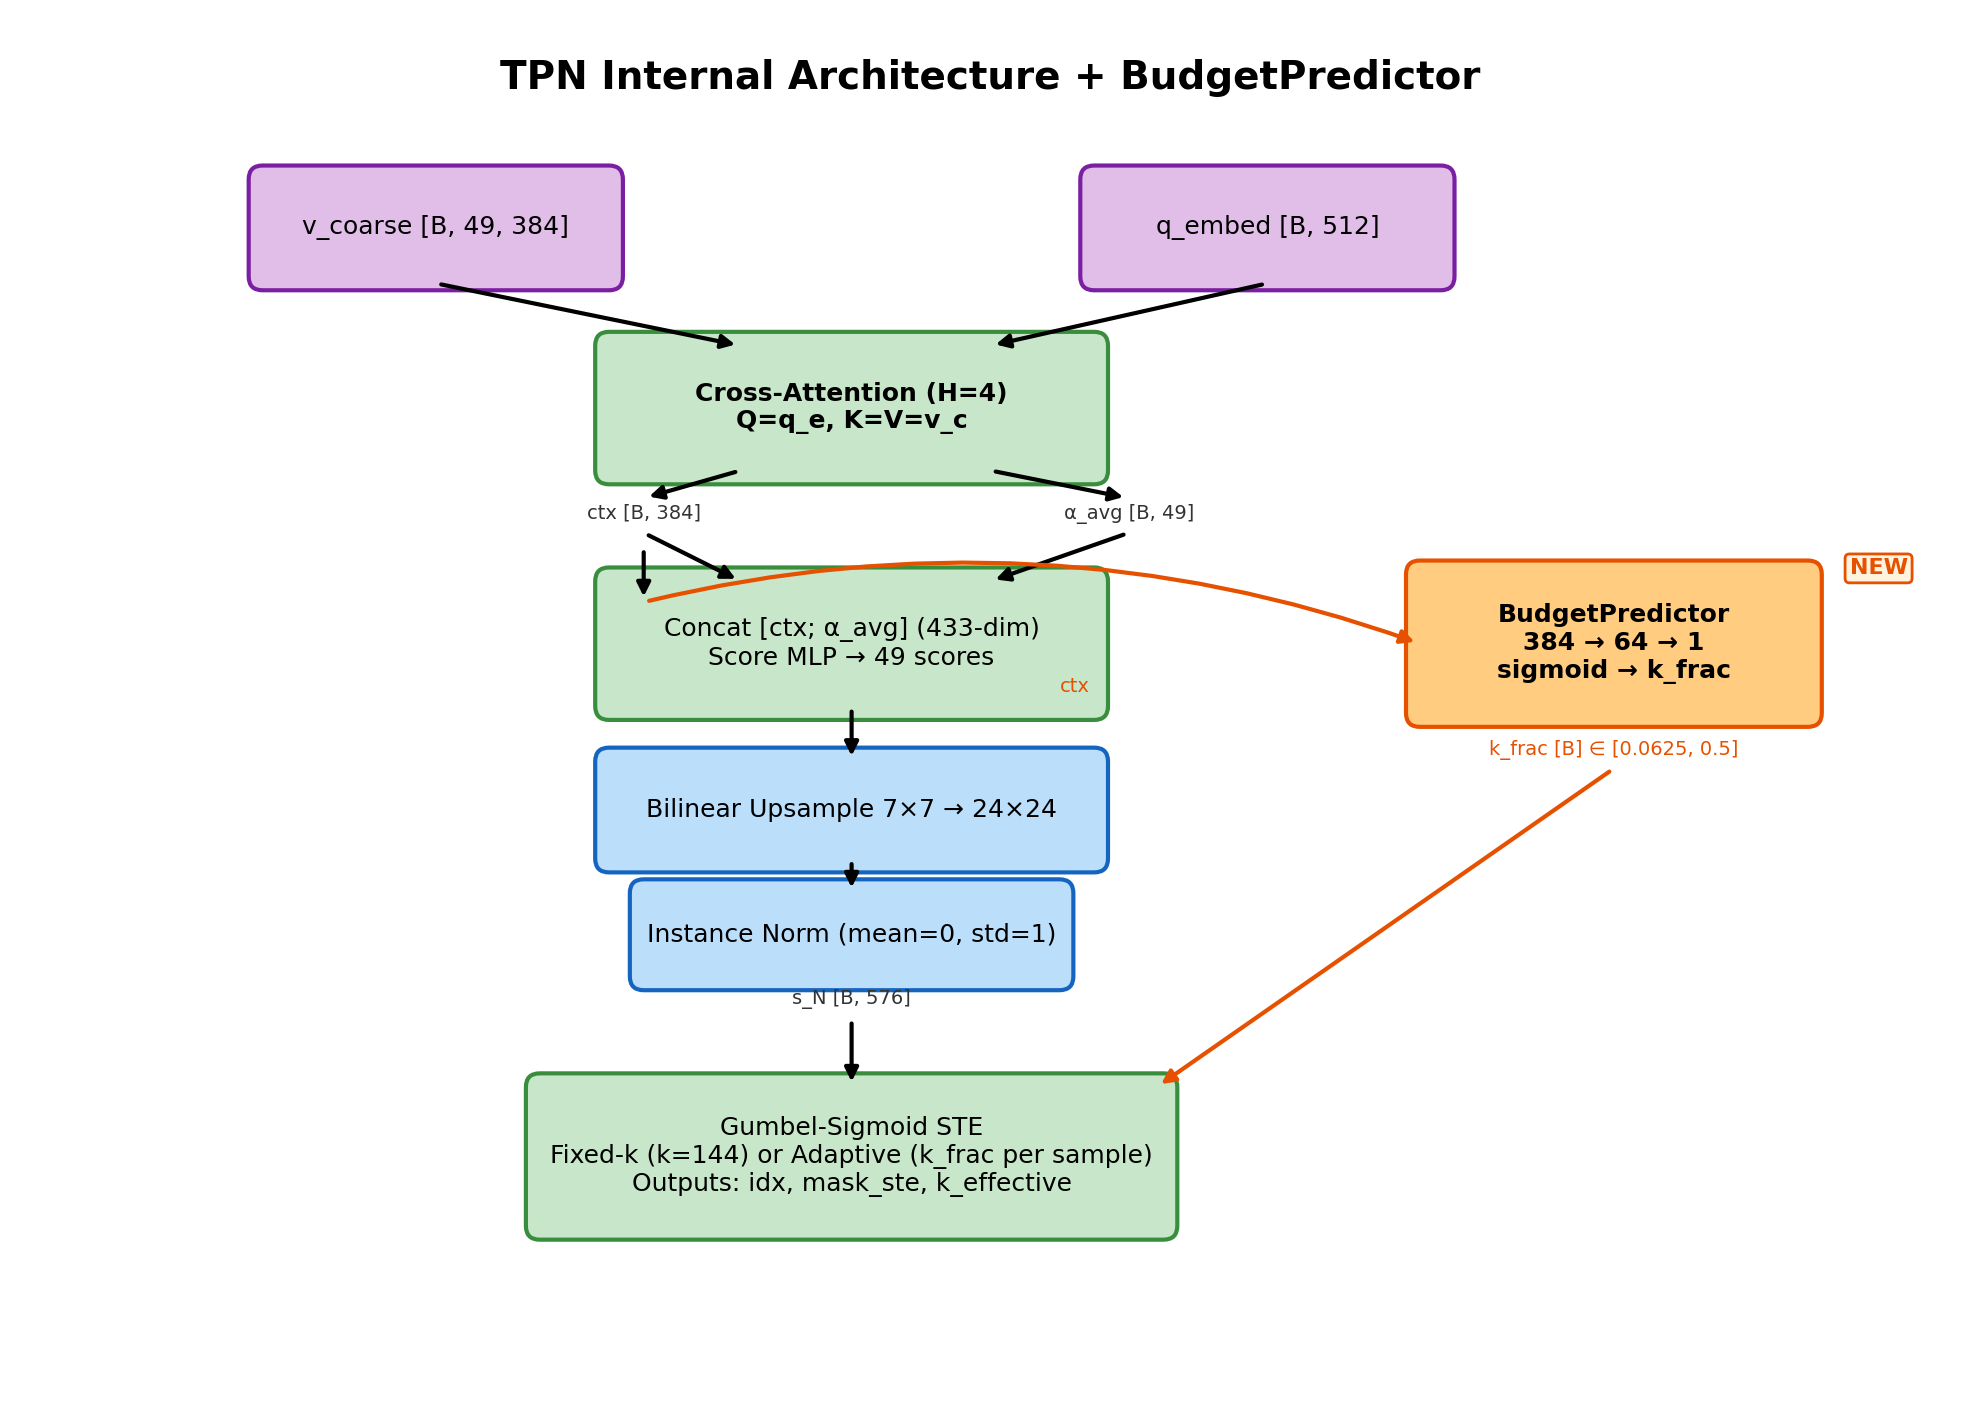
\includegraphics[width=0.92\columnwidth]{figures/tpn_architecture.png}
\caption{\textbf{TPN internal architecture and BudgetPredictor wiring.}
Cross-attention with $H{=}4$ heads ($Q{=}\qemb$, $K{=}V{=}\vcoarse$) produces a
context vector $\mathrm{ctx}{\in}\mathbb{R}^{384}$ and head-averaged spatial
weights $\boldsymbol{\alpha}{\in}\mathbb{R}^{49}$.
The $[\mathrm{ctx};\boldsymbol{\alpha}]$ concatenation passes through a Score MLP
producing 49 coarse scores, which are bilinearly upsampled $7{\times}7\to24{\times}24$
and instance-normalized to yield $\sN{\in}\mathbb{R}^{576}$.
Phase 1 Adaptive shares $\mathrm{ctx}$ with the BudgetPredictor (orange) which
emits the per-sample token fraction $k_{\mathrm{frac}}{\in}[0.0625, 0.5]$
consumed by the Adaptive Gumbel-STE.}
\label{fig:tpn}
\end{figure}

\subsection{Gumbel-Sigmoid Straight-Through Estimator}
\label{sec:ste}

Token selection is a discrete top-$k$ operation with zero gradients almost everywhere.
We adapt the Gumbel-Sigmoid STE~\cite{jang2017categorical, bengio2013estimating}
for independent binary subset selection over 576 positions.

\textbf{Forward pass.} Gumbel noise $\mathbf{g} \sim \mathrm{Gumbel}(0,1)$ provides
per-sample diversity; the temperature $\tau$ controls the soft-to-hard transition:
\begin{align}
  \mathbf{n} &= \sN + \mathbf{g}, \label{eq:noisy} \\
  \mathbf{m}_{\mathrm{soft}} &= \sigma(\mathbf{n} / \tau) \in (0,1)^N, \label{eq:soft} \\
  \text{idx} &= \mathrm{topk}(\mathbf{n},\, k), \label{eq:topk} \\
  \mathbf{m}_{\mathrm{hard}} &= \mathbf{0};\; \mathbf{m}_{\mathrm{hard}}[\text{idx}] = 1, \label{eq:hard} \\
  \mathbf{m}_{\mathrm{STE}} &= \mathbf{m}_{\mathrm{hard}}
    - \mathbf{m}_{\mathrm{soft}}.\mathrm{detach}()
    + \mathbf{m}_{\mathrm{soft}}. \label{eq:ste}
\end{align}
In the forward pass, $\mathbf{m}_{\mathrm{STE}} = \mathbf{m}_{\mathrm{hard}}$
(the $\mathbf{m}_{\mathrm{soft}}$ terms cancel).
In the backward pass, the gradient flows through $\mathbf{m}_{\mathrm{soft}}$.
Noise in Eq.~\eqref{eq:noisy} (not raw scores) is used for top-$k$
to ensure per-sample selection diversity across the batch;
using raw scores selects identical positions for all samples, collapsing entropy.
Temperature is annealed linearly $\tau: 1.0 \to 0.3$ over training.

\textbf{Tau-independent additive gradient correction.}
At low $\tau$, $\mathbf{m}_{\mathrm{soft}}$ saturates toward $\{0,1\}$, making
$\partial \mathbf{m}_{\mathrm{soft}} / \partial \sN \approx 0$ for all
positions with $|\sN[i]| > 1$.
This kills the gradient path to TPN weights, halting learning after $\tau$
has annealed.
We resolve this by multiplying gathered visual tokens by an additive correction:
\begin{equation}
  \vsel = \mathrm{gather}(\vfine, \text{idx}), \quad
  \mathbf{c} = \mathrm{gather}(\sN, \text{idx}), \label{eq:gather}
\end{equation}
\begin{align}
  \vsel &\leftarrow \vsel \odot \bigl(1 + \mathbf{c} - \mathbf{c}.\mathrm{detach}()\bigr).
  \label{eq:taufix}
\end{align}
In the forward pass, $\mathbf{c} - \mathbf{c}.\mathrm{detach}() = \mathbf{0}$,
so $\vsel$ is unchanged.
In the backward pass, for selected position $j$:
\[
  \frac{\partial \mathcal{L}_\mathrm{VQA}}{\partial \sN[j]}
  = \sum_{d=1}^{D_v} \frac{\partial \mathcal{L}}{\partial \vsel[j,d]} \cdot \vsel[j,d],
\]
a dot product between the VQA gradient and visual features at position $j$.
This gradient is non-zero at any $\tau$ and provides a dense, token-level
supervision signal for TPN throughout training.

\begin{figure*}[t]
\centering
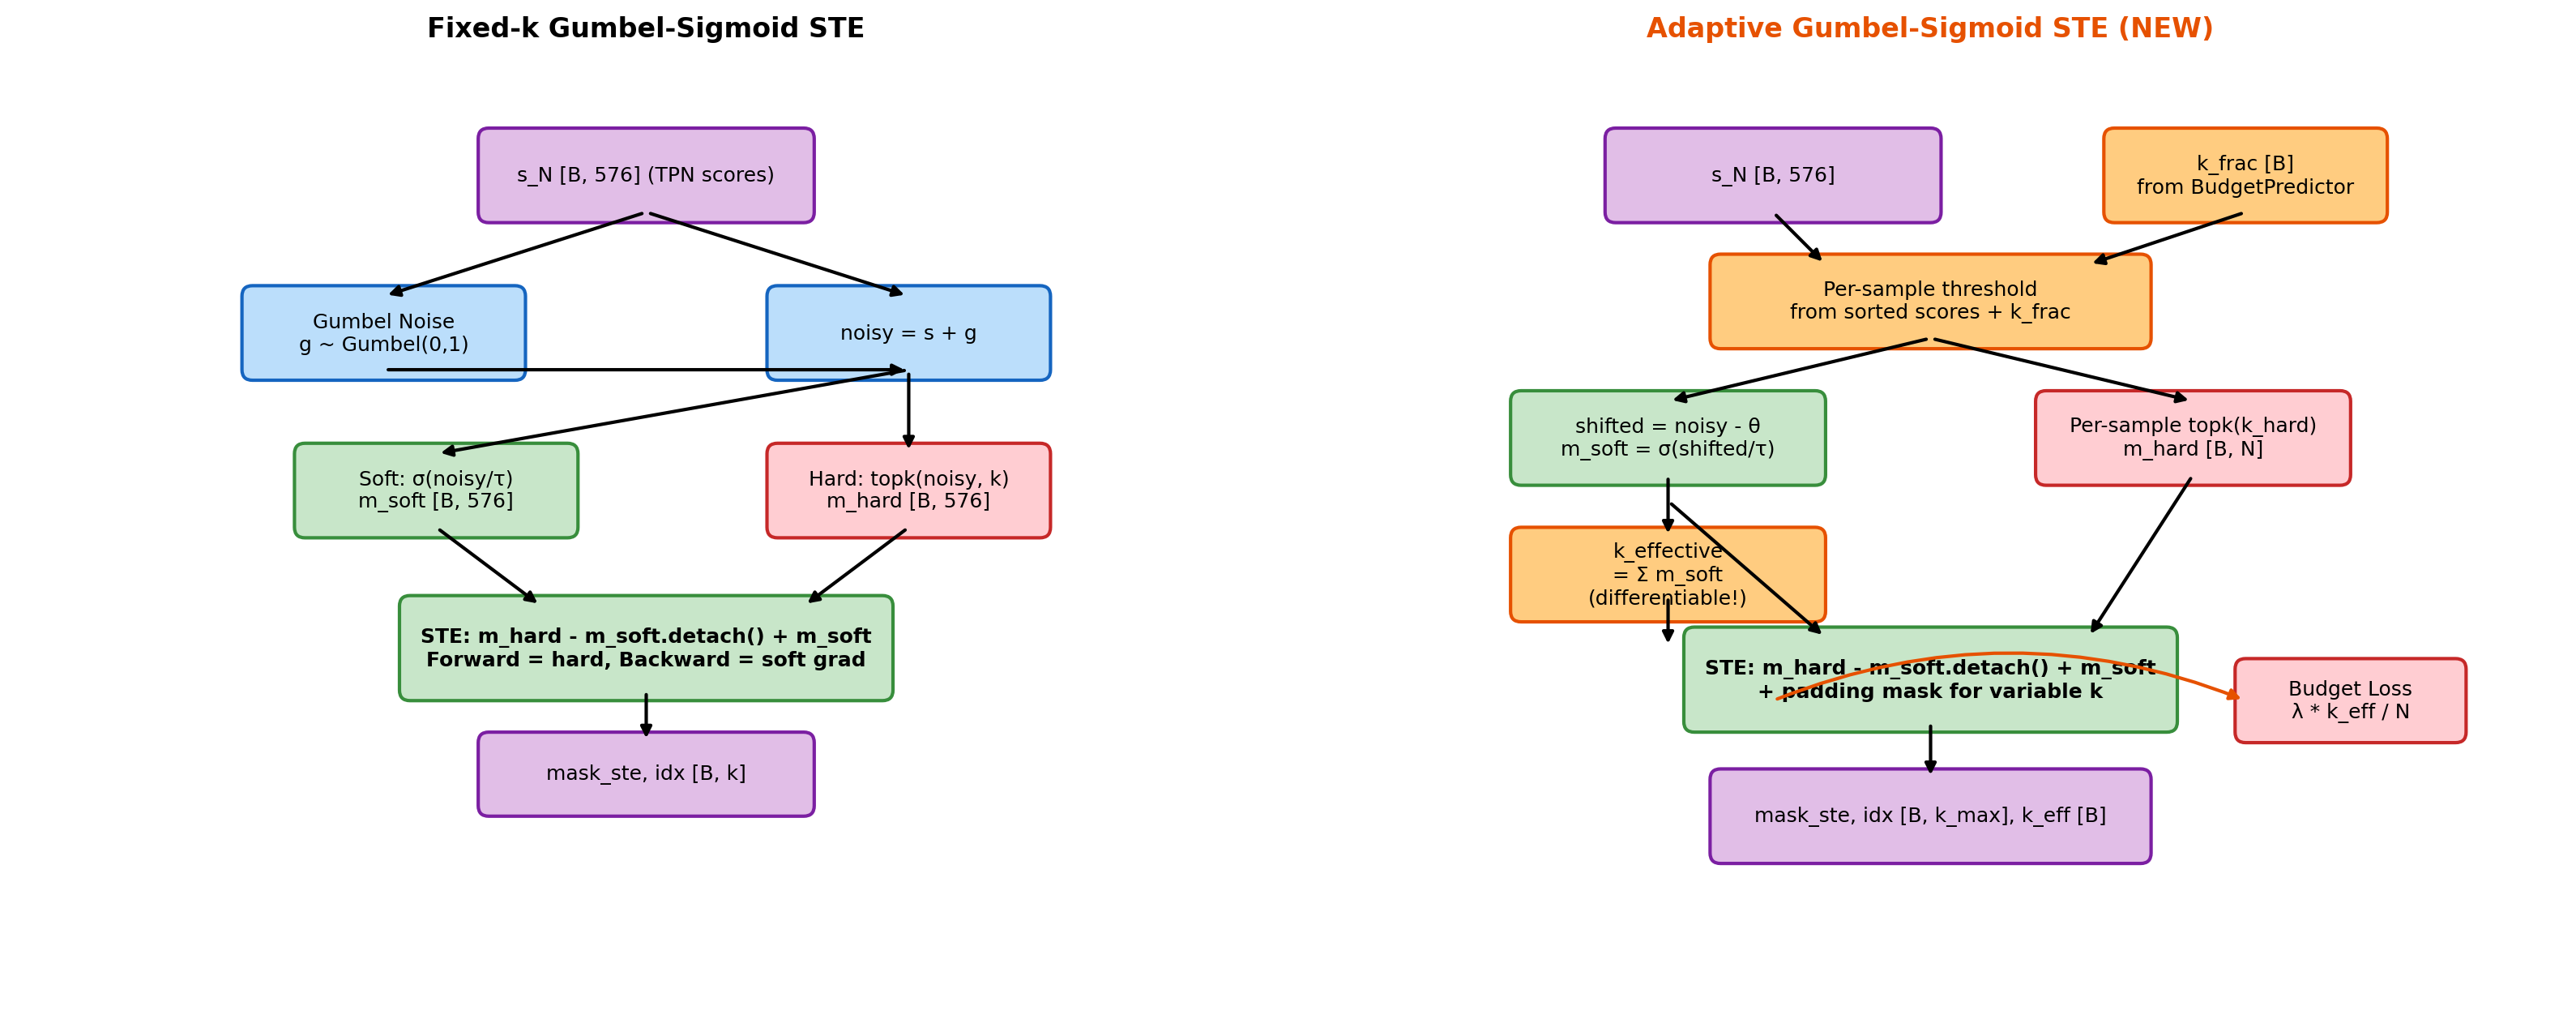
\includegraphics[width=0.96\textwidth]{figures/gumbel_ste.png}
\caption{\textbf{Fixed-$k$ vs.\ Adaptive Gumbel-Sigmoid STE} (Phase 1 Final vs.\
Phase 1 Adaptive). \emph{Left:} the standard fixed-budget pipeline: scores +
Gumbel noise feed both a soft sigmoid (for backward pass) and a hard top-$k{=}144$
selection (for forward pass), composed via the STE identity
$\mathbf{m}_{\mathrm{STE}}{=}\mathbf{m}_{\mathrm{hard}}{-}\mathbf{m}_{\mathrm{soft}}.\mathrm{detach}(){+}\mathbf{m}_{\mathrm{soft}}$.
\emph{Right:} the adaptive variant inserts a per-sample threshold $\theta$
derived from the BudgetPredictor's $k_{\mathrm{frac}}$ output. The shifted
soft mask $\sigma((\mathbf{n}{-}\theta)/\tau)$ produces a differentiable
effective count $k_{\mathrm{eff}}{=}\sum_i m_{\mathrm{soft},i}$ that drives
the budget loss; per-sample top-$k_{\mathrm{hard}}$ provides the hard mask
with right-padding to $k_{\max}$ for batched processing.}
\label{fig:ste}
\end{figure*}

\begin{figure}[t]
\centering
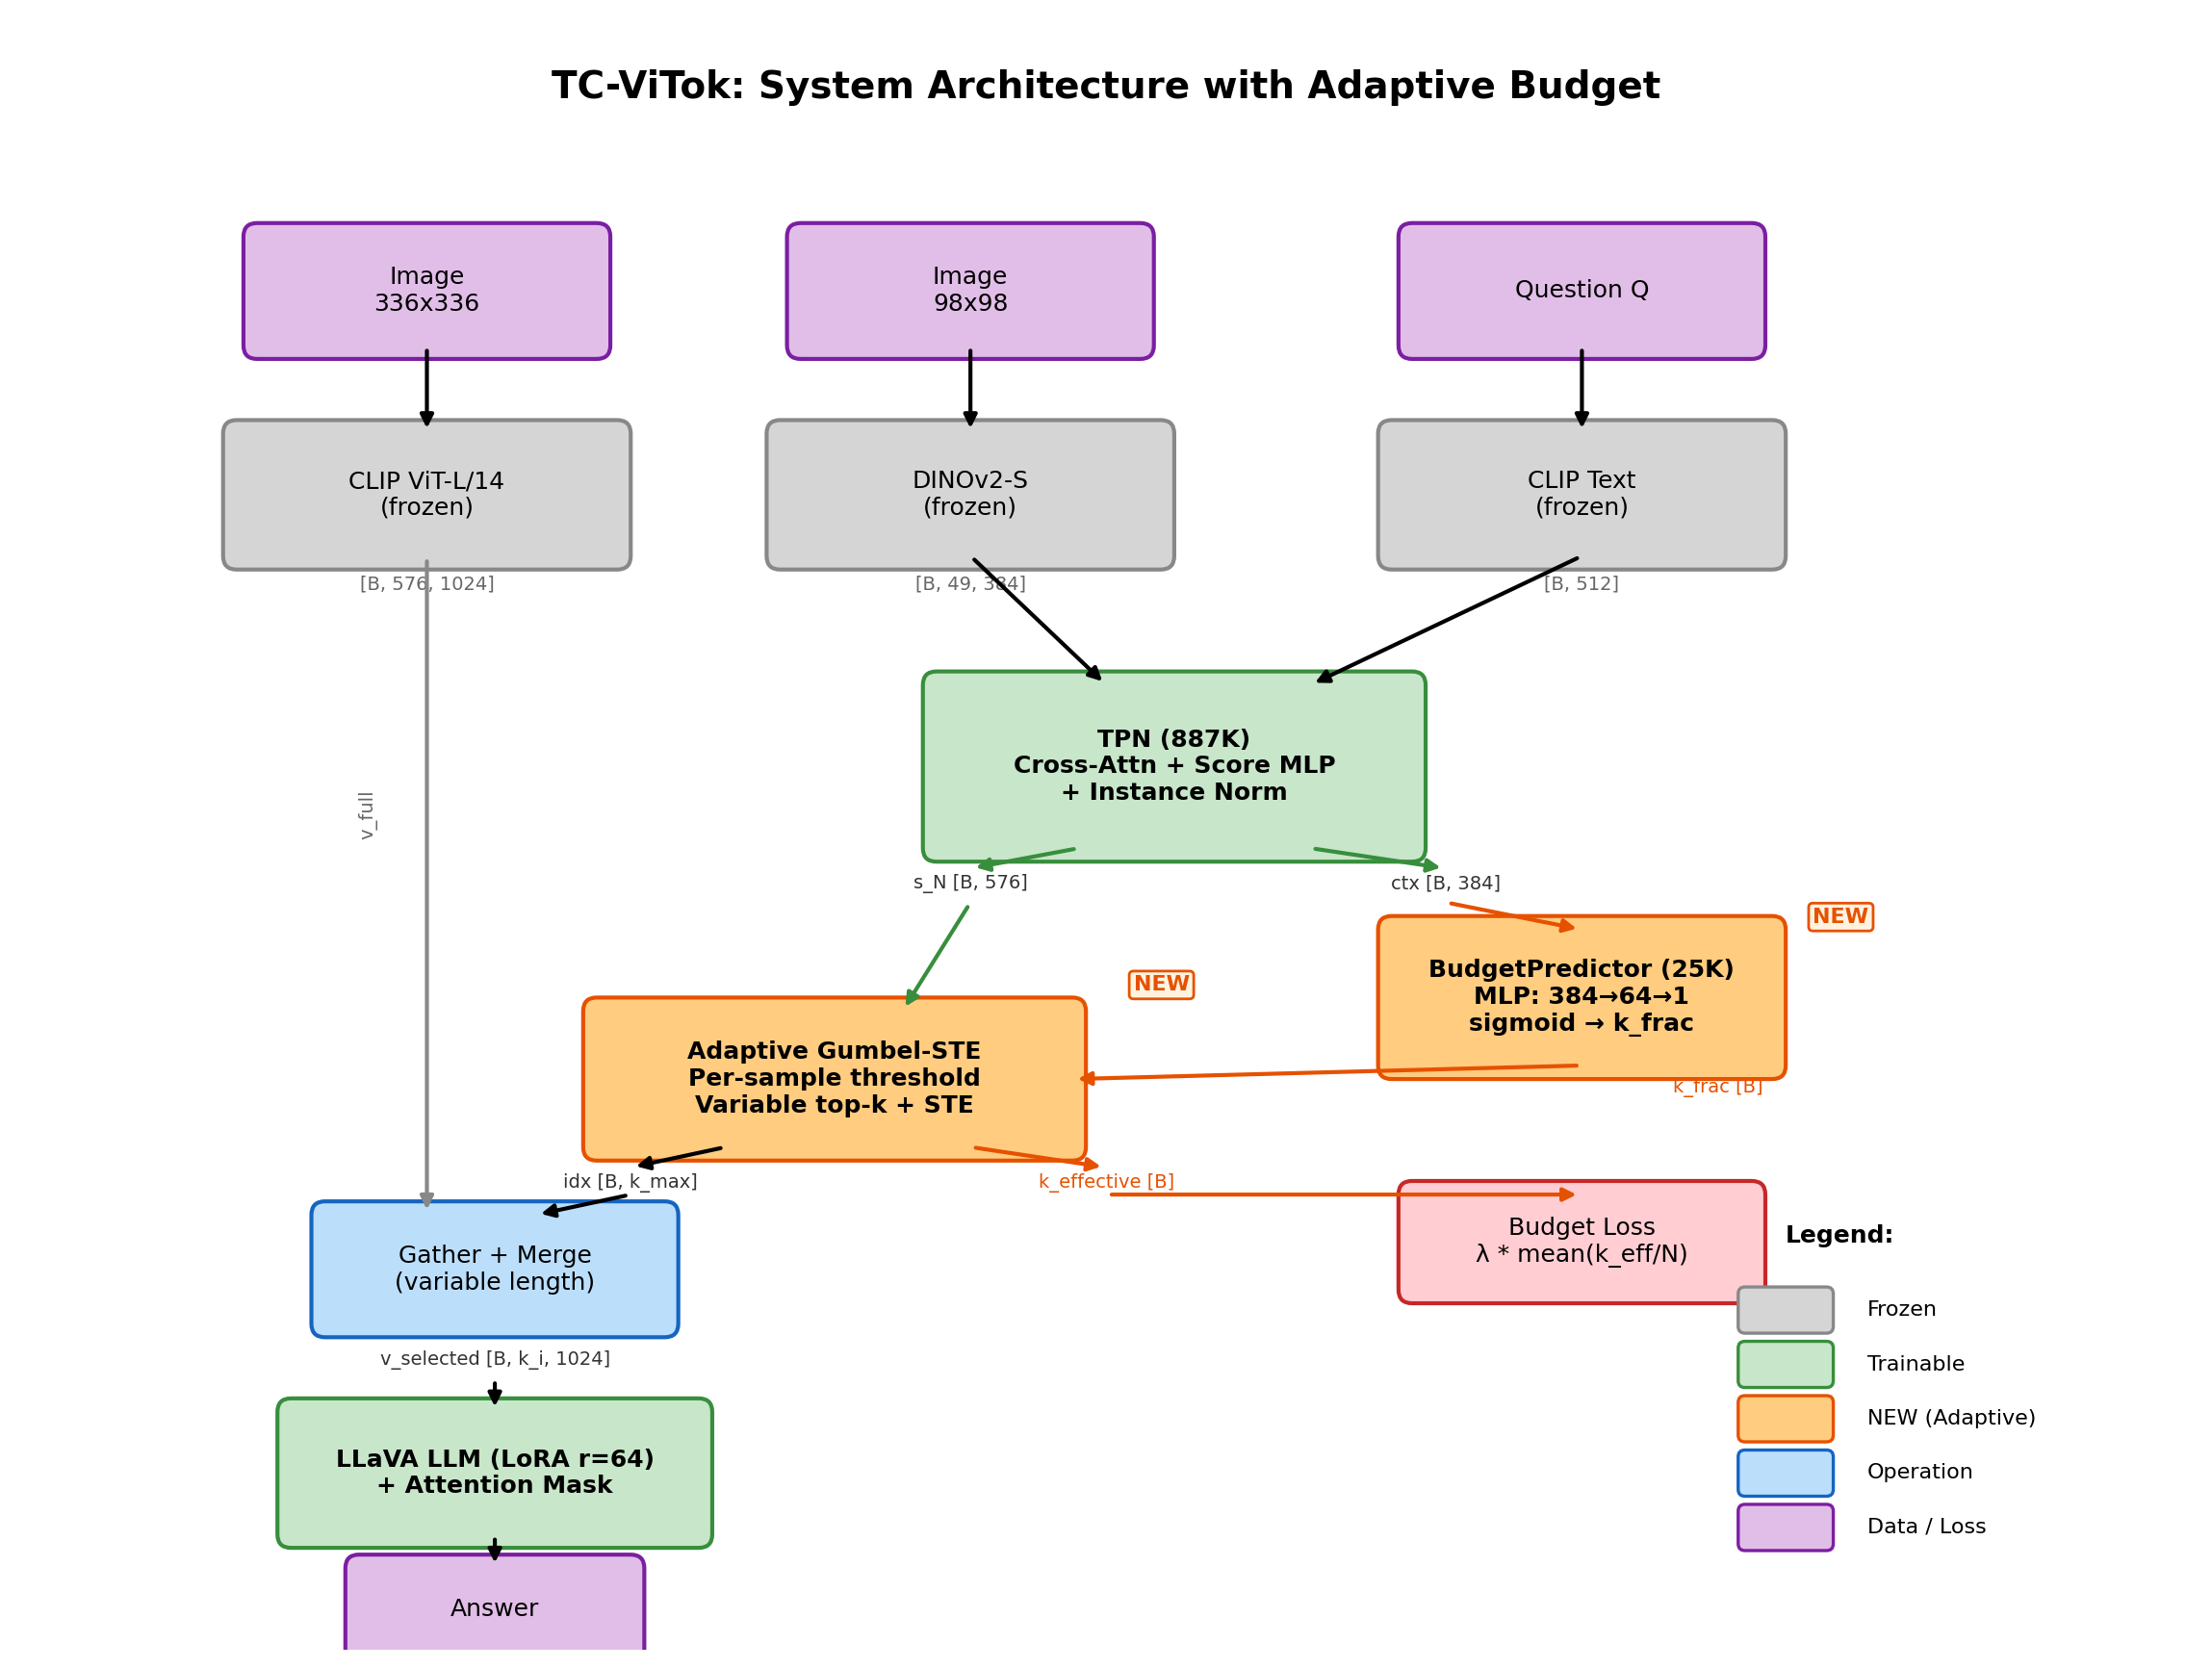
\includegraphics[width=0.95\columnwidth]{figures/tc_vitok_architecture.png}
\caption{\textbf{TC-ViTok system architecture with adaptive budget.}
Three frozen encoders (purple) extract complementary representations:
CLIP ViT-L/14 produces high-resolution patch tokens $\vfine$ for the LLM,
DINOv2-S provides a coarse spatial map $\vcoarse$ for the TPN, and
CLIP Text encodes the question into $\qemb$.
The TPN (887K) cross-attends $\qemb$ over $\vcoarse$ and emits per-position
scores $\sN$ plus a context vector $\mathrm{ctx}$. In adaptive mode, the
BudgetPredictor (25K, orange) maps $\mathrm{ctx}$ to a per-sample token fraction.
The Adaptive Gumbel-STE produces variable-length selection indices, which
gate-and-merge $\vfine$ before the multimodal projector and LLaVA-1.5-7B+LoRA.}
\label{fig:arch}
\end{figure}

\subsection{Informative Token Merge}
\label{sec:merge}

Hard dropping of the 432 unselected tokens discards all the contextual information
they carry.
PruMerge~\cite{shang2024llava} shows that merging such tokens recovers $\sim$2\%
VQAv2 over pure pruning at the same budget.
We implement a query-conditioned variant: the TPN score of an unselected token
determines how strongly it contributes to the merge, so tokens that were ``almost
selected'' (near-threshold, task-relevant) contribute more than distant background tokens.

Let $\vsel \in \mathbb{R}^{k \times D_v}$ be the gathered selected tokens and
$\vunsel \in \mathbb{R}^{(N-k) \times D_v}$ the unselected tokens.
Each unselected token $i$ is soft-assigned to the nearest selected token by cosine similarity:
\begin{equation}
  A_{ij} = \mathrm{softmax}_j
  \!\left(\frac{\hat{\mathbf{v}}_{\mathrm{unsel},i}^\top \hat{\mathbf{v}}_{\mathrm{sel},j}}
               {\tau_m}\right), \label{eq:assign}
\end{equation}
where $\hat{\cdot}$ denotes $\ell_2$-normalization and $\tau_m{=}0.1$.
Each unselected token is further weighted by its TPN score:
\begin{equation}
  w_i = \mathrm{softmax}_i(s_i^{\mathrm{unsel}}), \label{eq:scoreweight}
\end{equation}
where $s_i^{\mathrm{unsel}} = \sN[\mathrm{unsel\_idx}[i]]$.
The normalized contribution matrix $\tilde{A}_{ij} = w_i A_{ij} /
\!\sum_{i'} w_{i'} A_{i'j}$ aggregates unselected content into each selected token:
\begin{equation}
  \vmerged = \vsel + \beta \cdot \tilde{A}^\top \vunsel, \quad \beta = 0.3.
  \label{eq:merge}
\end{equation}

This mechanism introduces zero new parameters, eliminates any co-adaptation risk with LoRA,
and preserves the exact token count $k$ between training and evaluation (avoiding the
train-eval mismatch that corrupted our earlier trainable pooler experiments).

\begin{figure}[t]
\centering
\resizebox{\columnwidth}{!}{%
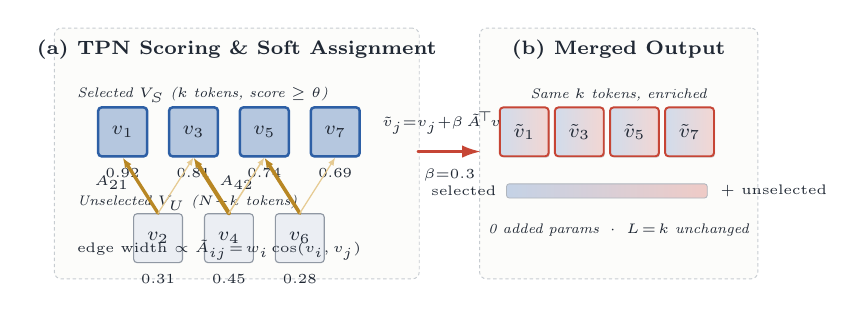
\begin{tikzpicture}[
    every node/.style={font=\scriptsize, text=tcink},
    sel/.style={rectangle, draw=tcblue, fill=tcbluelight, line width=0.6pt,
                minimum width=0.62cm, minimum height=0.62cm,
                inner sep=0pt, rounded corners=1.2pt,
                font=\scriptsize\bfseries\color{tcblue}, text centered},
    selhi/.style={sel, fill=tcblue!35, draw=tcblue, line width=0.9pt,
                  font=\scriptsize\bfseries\color{tcink},
                  drop shadow={shadow xshift=0.3pt, shadow yshift=-0.4pt,
                               opacity=0.18, fill=tcink}},
    unsel/.style={rectangle, draw=tcgray!70, fill=tcgraylight, line width=0.4pt,
                  minimum width=0.62cm, minimum height=0.62cm,
                  inner sep=0pt, rounded corners=1.2pt,
                  font=\scriptsize\color{tcgray!90!black}, text centered},
    merged/.style={rectangle, draw=tcaccent, line width=0.7pt,
                   left color=tcblue!22, right color=tcaccent!22,
                   minimum width=0.62cm, minimum height=0.62cm,
                   inner sep=0pt, rounded corners=1.2pt,
                   font=\scriptsize\bfseries\color{tcink}, text centered,
                   drop shadow={shadow xshift=0.4pt, shadow yshift=-0.5pt,
                                opacity=0.20, fill=tcink}},
    panellbl/.style={font=\scriptsize\bfseries\color{tcink}, align=center},
    sublbl/.style={font=\tiny\itshape\color{tcgray}},
    sectionbg/.style={rectangle, rounded corners=2.5pt,
                      draw=tcgray!35, line width=0.35pt,
                      fill=tcpaper, dashed, dash pattern=on 1.2pt off 1pt},
    asgn/.style={->, >={Latex[length=1.3mm,width=1.0mm]}, draw=tcgold!90!black, line cap=round},
    asgnweak/.style={->, >={Latex[length=1.0mm,width=0.8mm]}, draw=tcgold!50, line cap=round, line width=0.25pt},
    flowarr/.style={-{Latex[length=2.4mm,width=1.6mm]},
                    line width=1.0pt, draw=tcaccent, line cap=round},
]

% ============== Panel A background ==============
\begin{scope}[on background layer]
  \node[sectionbg, fit={(-0.45,-0.30) (3.95,2.65)}] {};
\end{scope}
\node[panellbl] at (1.75, 2.50) {(a) TPN Scoring \& Soft Assignment};

% ----- selected row -----
\node[sublbl, anchor=west] at (-0.40, 1.92)
     {Selected $V_S$ ($k$ tokens, score $\geq \theta$)};
\node[selhi]   (s1) at (0.30, 1.45) {$v_1$};
\node[selhi]   (s2) at (1.20, 1.45) {$v_3$};
\node[selhi]   (s3) at (2.10, 1.45) {$v_5$};
\node[selhi]   (s4) at (3.00, 1.45) {$v_7$};
% scores under selected
\foreach \nn/\val in {s1/0.92, s2/0.81, s3/0.74, s4/0.69} {
  \node[font=\tiny\color{tcblue!85!black}, anchor=north, yshift=-0.5pt]
       at (\nn.south) {\val};
}

% ----- unselected row -----
\node[sublbl, anchor=west] at (-0.40, 0.55)
     {Unselected $V_U$ ($N{-}k$ tokens)};
\node[unsel]   (u1) at (0.75,  0.10) {$v_2$};
\node[unsel]   (u2) at (1.65,  0.10) {$v_4$};
\node[unsel]   (u3) at (2.55,  0.10) {$v_6$};
% scores under unselected
\foreach \nn/\val in {u1/0.31, u2/0.45, u3/0.28} {
  \node[font=\tiny\color{tcgray!90!black}, anchor=north, yshift=-0.5pt]
       at (\nn.south) {\val};
}

% ----- assignment edges (thickness ∝ cos sim × score) -----
\draw[asgn,     line width=1.2pt] (u1.north) -- (s1.south)
      node[pos=0.55, left=-0.5pt, font=\tiny\color{tcgold!75!black}]{$A_{21}$};
\draw[asgnweak, line width=0.45pt] (u1.north) -- (s2.south);
\draw[asgn,     line width=1.5pt] (u2.north) -- (s2.south)
      node[pos=0.55, right=-0.5pt, font=\tiny\color{tcgold!75!black}]{$A_{42}$};
\draw[asgnweak, line width=0.55pt] (u2.north) -- (s3.south);
\draw[asgn,     line width=1.3pt] (u3.north) -- (s3.south);
\draw[asgnweak, line width=0.45pt] (u3.north) -- (s4.south);

% legend strip for assignment thickness
\node[font=\tiny\color{tcgold!75!black}, anchor=west]
     at (-0.40, -0.05) {edge width $\propto \tilde{A}_{ij}\!=\!w_i\,\mathrm{cos}(v_i,v_j)$};

% ============== flow arrow ==============
\draw[flowarr] (4.05, 1.20) -- (4.85, 1.20);
\node[font=\tiny\color{tcaccent}, align=center, anchor=south]
     at (4.45, 1.30) {$\tilde{v}_j {=} v_j {+}\beta\,\tilde{A}^{\!\top}\!v_U$};
\node[font=\tiny\color{tcgray}, align=center, anchor=north]
     at (4.45, 1.10) {$\beta{=}0.3$};

% ============== Panel B background ==============
\begin{scope}[on background layer]
  \node[sectionbg, fit={(4.95,-0.30) (8.25,2.65)}] {};
\end{scope}
\node[panellbl] at (6.60, 2.50) {(b) Merged Output};

\node[sublbl, anchor=center] at (6.60, 1.92)
     {Same $k$ tokens, enriched};
\node[merged] (m1) at (5.40, 1.45) {$\tilde{v}_1$};
\node[merged] (m2) at (6.10, 1.45) {$\tilde{v}_3$};
\node[merged] (m3) at (6.80, 1.45) {$\tilde{v}_5$};
\node[merged] (m4) at (7.50, 1.45) {$\tilde{v}_7$};

% small gradient bar below to indicate "selected + absorbed unselected"
\node[draw=tcgray!50, line width=0.3pt, rectangle, rounded corners=1pt,
      left color=tcblue!28, right color=tcaccent!28,
      minimum width=2.55cm, minimum height=0.18cm,
      inner sep=0pt] (gradbar) at (6.45, 0.70) {};
\node[font=\tiny\color{tcblue!85!black}, anchor=east] at (gradbar.west) {selected};
\node[font=\tiny\color{tcaccent}, anchor=west] at (gradbar.east) {\,+ unselected};

\node[sublbl, anchor=center, align=center] at (6.60, 0.20)
     {0 added params \;$\cdot$\; $L\!=\!k$ unchanged};

\end{tikzpicture}%
}
\caption{\textbf{Informative Token Merge (parameter-free).}
\textbf{(a)} Each unselected token (gray) is soft-assigned to the most similar
selected token (blue) via cosine similarity. Edge thickness encodes
$\tilde{A}_{ij}{=}w_i\,\cos(v_i,v_j)$, where $w_i$ is the unselected token's TPN score
(numbers below each token).
\textbf{(b)} Merged outputs (gradient: selected~$\to$~unselected) preserve sequence length~$k$ but absorb background context from all $N{-}k$ discarded tokens. No new parameters.}
\label{fig:merge}
\end{figure}

\subsection{Adaptive Budget}
\label{sec:adaptive}

The fixed $k{=}144$ model compresses all images equally.
We extend TC-ViTok with a \emph{BudgetPredictor} that learns per-sample token fractions.

\textbf{BudgetPredictor architecture ($\approx$25K params).}
\begin{align}
  k_{\mathrm{frac}} = \sigma\Bigl(
    &\mathrm{Lin}_{64 \to 1}\bigl(\mathrm{GELU}\bigl(
      \mathrm{Lin}_{385 \to 64}([\mathrm{ctx};\, \bar{h}(\sN)])
    \bigr)\bigr)
  \Bigr), \label{eq:bp}
\end{align}
where $\mathrm{ctx} \in \mathbb{R}^{384}$ is the TPN's attended visual context vector
(encoding which visual regions are relevant to the question),
$\bar{h}(\sN) \in \mathbb{R}^{1}$ is the normalized entropy of $\sN$
(a measure of how focused the importance distribution is),
and $\sigma$ clips the output to $[k_{\min}/N,\, k_{\max}/N] = [36/576,\, 288/576]$.

\textbf{Differentiable threshold.}
Converting $k_{\mathrm{frac}}$ to a hard selection requires a discrete step:
$k_{\mathrm{hard}} = \lfloor k_{\mathrm{frac}} \cdot N \rceil$.
To route gradients from the budget penalty to the predictor despite this
non-differentiability, we define a modified threshold:
\begin{align}
  \theta &= \theta_{\mathrm{hard}}
    - \bigl(k_{\mathrm{target}} - k_{\mathrm{target}}.\mathrm{detach}()\bigr),
  \label{eq:thresh}
\end{align}
where $k_{\mathrm{target}} = k_{\mathrm{frac}} \cdot N$ and
$\theta_{\mathrm{hard}}$ is the score at position $k_{\mathrm{hard}}$
in the sorted score sequence (no gradient).
In the forward pass, Eq.~\eqref{eq:thresh} evaluates to $\theta_{\mathrm{hard}}$
(the correction is zero).
In the backward pass, $\partial\theta/\partial k_{\mathrm{frac}} = -N$,
providing a non-zero gradient to the BudgetPredictor from the budget penalty loss.
The shifted soft mask $\sigma((\mathbf{n} - \theta)/\tau)$
produces a differentiable effective count $k_{\mathrm{eff}} = \sum_i m_{\mathrm{soft},i}$
used in the loss; hard selection uses per-sample $\mathrm{topk}(k_{\mathrm{hard}})$.

\textbf{Budget penalty loss.}
$\mathcal{L}_{\mathrm{budget}} = \lambda_b \cdot \mathbb{E}[k_{\mathrm{eff}} / N]$
penalizes using more tokens.
Higher $\lambda_b$ forces fewer tokens but risks accuracy degradation.
We sweep $\lambda_b \in \{0.05, 0.1, 0.2, 0.4\}$ to trace the Pareto frontier.

\subsection{Loss Functions}
\label{sec:loss}

The total training loss is:
\begin{equation}
  \mathcal{L} = \mathcal{L}_\mathrm{VQA}
              + \lambda_H (-H)
              + \lambda_d \mathcal{L}_\mathrm{div}
              + \lambda_b \mathcal{L}_\mathrm{budget}, \label{eq:loss}
\end{equation}
where $\mathcal{L}_\mathrm{VQA}$ is the next-token prediction cross-entropy on answer
tokens (labels $=-100$ for visual/question tokens), $H$ is the spatial entropy of
the batch-mean selection distribution, and $\mathcal{L}_\mathrm{div}$ is a diversity
loss.
Table~\ref{tab:loss} summarizes each term.

\begin{table}[t]
\caption{Loss function components.}
\label{tab:loss}
\vskip 0.1in
\centering
\begin{small}
\begin{tabular}{llc}
\toprule
\textbf{Term} & \textbf{Purpose} & \textbf{Weight} \\
\midrule
$\mathcal{L}_\mathrm{VQA}$ & NTP cross-entropy on answer tokens & 1.0 \\
$-H$ & Prevent spatial collapse of TPN & 0.02 \\
$\mathcal{L}_\mathrm{div}$ & Prevent query-ignoring & 0.1 \\
$\mathcal{L}_\mathrm{budget}$ & Penalize token usage (Phase 1-Adap.) & sweep \\
\bottomrule
\end{tabular}
\end{small}
\end{table}

\textbf{Spatial entropy ($-H$).}
Without this term, TPN quickly focuses all selections on a fixed spatial region (the image
center, which is most discriminative in VQAv2).
$H = -\sum_i p_i \log p_i$ where $\mathbf{p}$ is the normalized batch-mean selection
frequency; minimizing $-H$ maximizes distributional spread across positions.

\textbf{Diversity loss ($\mathcal{L}_\mathrm{div}$).}
Paired adjacent batch samples: $\mathcal{L}_\mathrm{div} = \mathbb{E}[\cos({\sN}_a,{\sN}_b) \cdot
(1 - \cos(\qemb_a, \qemb_b))]$.
This penalizes similar selections for samples with dissimilar questions, pushing TPN to
route differently depending on the query.

\subsection{Training Protocol}
\label{sec:training}

Training follows a three-phase curriculum where each phase adds one component.

\textbf{Phase 0 — TPN Warmup (10K steps).}
Only the TPN is trained; LLaVA's LLM, MM projector, and LoRA are frozen.
With LoRA frozen, the only way to reduce $\mathcal{L}_\mathrm{VQA}$ is through
better token selection — forcing TPN to learn meaningful query-conditioned scores
before joint co-training.
Temperature $\tau = 1.0$ (fixed); data: VQAv2 training split.

\textbf{Phase 1 Final — Joint Training with Token Merge (80K steps).}
TPN + LoRA (rank 64) + MM projector are co-trained.
LoRA is frozen for the first 3000 steps (\emph{warm-freeze}) to prevent it from
immediately compensating for TPN imperfections, preserving the gradient signal that
forces TPN to improve.
$\tau$ anneals $1.0 \to 0.3$; data: VQAv2 + GQA; effective batch size 128
($4 \times 16 \times 2$ GPUs).
Checkpoint loaded from Phase 0.

\textbf{Phase 1 Adaptive — Variable Budget Training (40K steps).}
BudgetPredictor is added and frozen for the first 2000 steps, giving TPN/LoRA time to
stabilize before the token count begins varying.
Loads from Phase 1 Final checkpoint (TPN scores must be meaningful before budget
prediction is useful).

\begin{figure}[t]
\centering
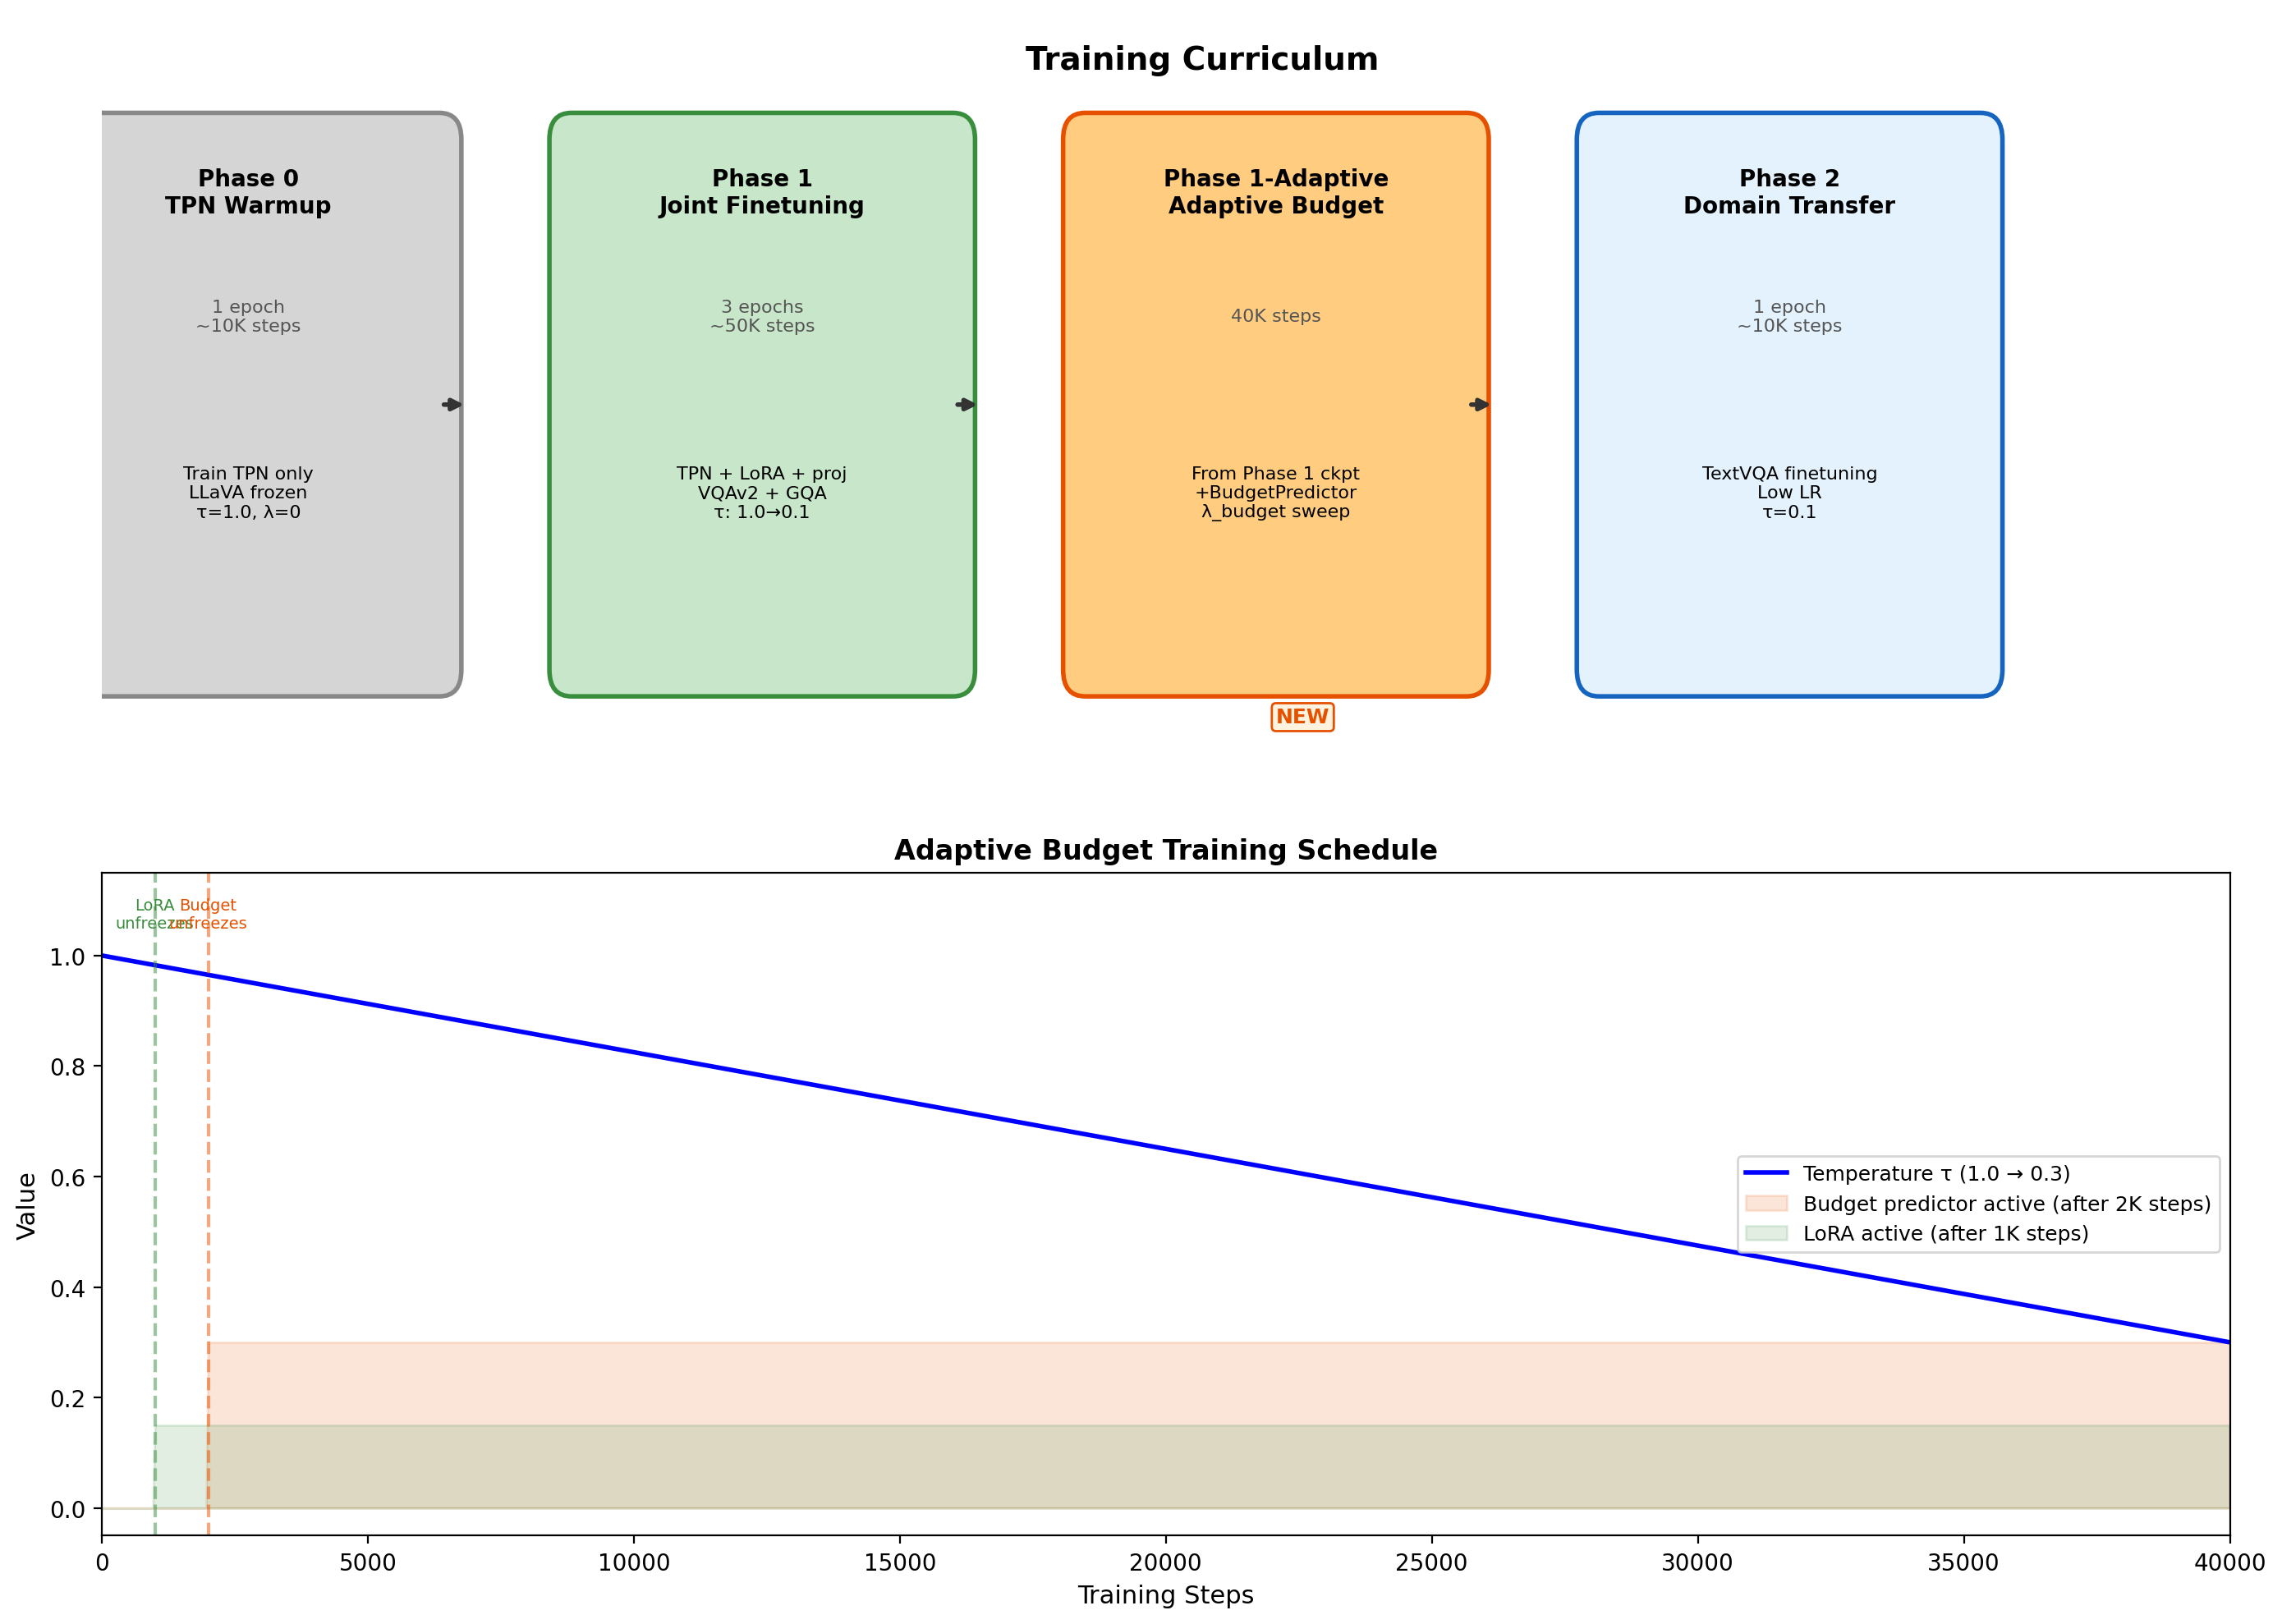
\includegraphics[width=0.97\columnwidth]{figures/training_pipeline.png}
\caption{\textbf{Training curriculum and adaptive-budget schedule.}
\emph{Top:} four phases trained sequentially. Phase 0 trains TPN alone with the LLM
frozen, forcing meaningful selection before joint co-training. Phase 1 unfreezes
LoRA + projector for joint fine-tuning. Phase 1-Adaptive (orange) loads from
Phase 1 Final and adds the BudgetPredictor with $\lambda_b$ sweep.
Phase 2 (domain transfer to TextVQA) is left as future work.
\emph{Bottom:} per-step temperature anneal $\tau{:}1.0{\to}0.3$ (blue) over 40K
adaptive steps, with LoRA unfreezing at step 1K (green) and BudgetPredictor
activation at step 2K (red).}
\label{fig:pipeline}
\end{figure}

\begin{table}[t]
\caption{Training hyperparameters per phase. P1-F = Phase 1 Final; P1-A = Phase 1
Adaptive. The expanded LoRA target set in P1-F (FFN layers) is critical — it
allows the LLM to adapt to merged token representations.}
\label{tab:hparam}
\vskip 0.1in
\centering
\begin{small}
\begin{tabular}{lccc}
\toprule
\textbf{Hyperparameter} & \textbf{Phase 0} & \textbf{Phase 1-F} & \textbf{Phase 1-A} \\
\midrule
Steps                  & 10K  & 80K  & 40K \\
LR (TPN)               & $1\mathrm{e}{-3}$ & $3\mathrm{e}{-3}$ & $1\mathrm{e}{-3}$ \\
LR (LoRA)              & —    & $1\mathrm{e}{-4}$ & $2\mathrm{e}{-4}$ \\
LR (MLP projector)     & —    & $5\mathrm{e}{-4}$ & $5\mathrm{e}{-4}$ \\
LR (BudgetPredictor)   & —    & —    & $1\mathrm{e}{-3}$ \\
LoRA rank / alpha      & —    & 64 / 128 & 64 / 128 \\
LoRA targets           & —    & q,k,v,o,\textbf{gate,up} & q,k,v,o \\
$\tau_{\max} \to \tau_{\min}$ & $1.0 \to 1.0$ & $1.0 \to 0.3$ & $1.0 \to 0.3$ \\
$\lambda_H$            & 0.01 & 0.02 & 0.02 \\
$\lambda_d$            & 0.0  & 0.1  & 0.1 \\
$\lambda_b$            & —    & —    & 0.1 \\
Data                   & VQAv2 & VQAv2+GQA & VQAv2+GQA \\
\bottomrule
\end{tabular}
\end{small}
\end{table}

% ===================================================================
\section{Efficiency Analysis}
\label{sec:efficiency}

The motivation for any token compression method is computational savings.
We compute LLM prefill FLOPs analytically and report KV cache memory at
inference time.
LLaMA-2-7B (the LLM backing LLaVA-1.5) has hidden dimension $d{=}4096$,
FFN inner dimension $d_{\mathrm{ff}}{=}11008$, and $L_{\mathrm{layer}}{=}32$ layers,
totaling $P{\approx}6.74$B parameters.

\textbf{Prefill FLOPs.}
For sequence length $L$, dense-layer FLOPs are well-approximated by
$2 \cdot L \cdot P$, with an additional $4 \cdot L^2 \cdot d \cdot L_{\mathrm{layer}}$
for the quadratic attention term~\cite{kaplan2020scaling}.
With visual + text + system tokens, the full LLaVA-1.5 sees $L{=}611$
($576 + 30 + 5$); TC-ViTok at $k{=}144$ sees $L{=}179$.
Substituting:
\[
\mathrm{FLOPs}_{\mathrm{full}} \approx 8.24 + 0.20 = 8.44 \text{ TFLOPs}
\]
\[
\mathrm{FLOPs}_{\mathrm{TC\text{-}ViTok}} \approx 2.41 + 0.02 = 2.43 \text{ TFLOPs}
\]
yielding a \textbf{$3.47{\times}$ LLM prefill speedup}.

\textbf{KV cache memory.}
Per-token KV cache size is $2 \cdot L_{\mathrm{layer}} \cdot d \cdot 2$ bytes
(BF16, K \& V) $= 0.5$~MB.
Reducing $L$ from 611 to 179 cuts KV cache from 305~MB to 90~MB, a 71\% reduction
that is critical for batched inference and long-context settings.

\textbf{Encoder-side overhead.}
The added DINOv2-S forward pass on a 98-pixel crop costs $\approx$3 GFLOPs
(0.04\% of LLM prefill); TPN forward is $\approx$90 MFLOPs (negligible);
token merge is $\approx$130 MFLOPs (cosine similarities and weighted sum).
Total TC-ViTok overhead: $\approx$3.2 GFLOPs, vs.\ a saving of $6.0$ TFLOPs
on the LLM —- a 1{:}1900 cost-benefit ratio.

\textbf{End-to-end inference.}
Adding the always-paid CLIP ViT-L/14 cost (80 GFLOPs):
full inference is 8.52 TFLOPs vs.\ TC-ViTok's 2.51 TFLOPs, a
\textbf{$3.39{\times}$ end-to-end speedup}.
Table~\ref{tab:flops} summarizes.

\begin{table}[t]
\caption{FLOPs and KV cache analysis on LLaVA-1.5-7B. Speedup is computed
relative to full LLaVA-1.5 inference. End-to-end includes the always-paid
CLIP ViT-L/14 encoder cost.}
\label{tab:flops}
\vskip 0.1in
\centering
\resizebox{\columnwidth}{!}{%
\begin{tabular}{lccc}
\toprule
\textbf{Component} & \textbf{Full (576)} & \textbf{TC-ViTok (144)} & \textbf{Reduction} \\
\midrule
LLM prefill (dense)   & 8.24 TF & 2.41 TF & $3.4{\times}$ \\
LLM prefill (attn $L^2$) & 0.20 TF & 0.02 TF & $10.0{\times}$ \\
DINOv2-S (added)      & — & 3.0 GF & — \\
TPN                   & — & 0.09 GF & — \\
Token Merge           & — & 0.13 GF & — \\
CLIP ViT-L/14 (always) & 80 GF & 80 GF & 1.0$\times$ \\
\midrule
\textbf{LLM prefill total} & \textbf{8.44 TF} & \textbf{2.43 TF} & $\mathbf{3.47\times}$ \\
\textbf{End-to-end total}  & \textbf{8.52 TF} & \textbf{2.51 TF} & $\mathbf{3.39\times}$ \\
\midrule
KV cache (BF16)        & 305 MB & 90 MB & 71\% smaller \\
\bottomrule
\end{tabular}%
}
\end{table}

\begin{figure}[t]
\centering
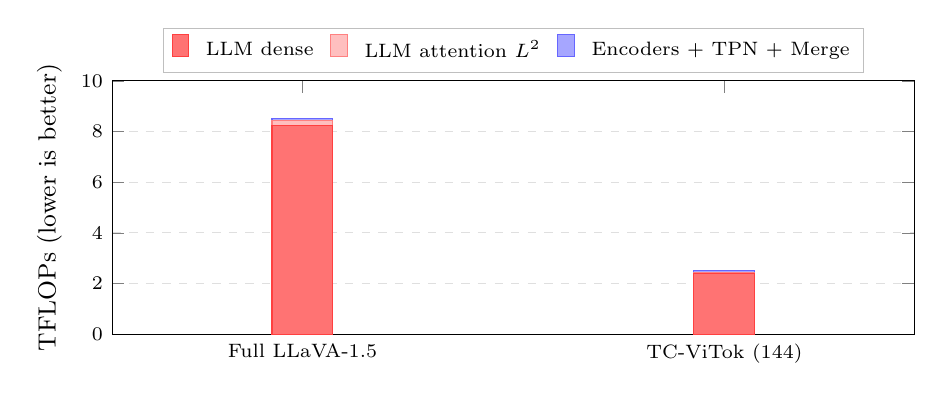
\begin{tikzpicture}
\begin{axis}[
  ybar stacked,
  width=0.97\columnwidth,
  height=4.8cm,
  bar width=22pt,
  symbolic x coords={Full LLaVA-1.5, TC-ViTok (144)},
  xtick=data,
  ymin=0, ymax=10,
  ylabel={TFLOPs (lower is better)},
  legend style={font=\scriptsize, at={(0.5,1.03)}, anchor=south,
                legend columns=3, column sep=4pt,
                fill=white, draw=gray!50},
  tick label style={font=\scriptsize},
  label style={font=\small},
  enlarge x limits=0.45,
  ymajorgrids=true,
  grid style={dashed,gray!25},
]
\addplot[fill=red!55, draw=red!75]
  coordinates {(Full LLaVA-1.5,8.24) (TC-ViTok (144),2.41)};
\addlegendentry{LLM dense}
\addplot[fill=red!25, draw=red!50]
  coordinates {(Full LLaVA-1.5,0.20) (TC-ViTok (144),0.02)};
\addlegendentry{LLM attention $L^2$}
\addplot[fill=blue!35, draw=blue!60]
  coordinates {(Full LLaVA-1.5,0.080) (TC-ViTok (144),0.083)};
\addlegendentry{Encoders + TPN + Merge}
\end{axis}
\end{tikzpicture}
\caption{Inference FLOPs breakdown. TC-ViTok delivers a $3.39\times$ end-to-end
speedup. The added encoder/TPN/merge overhead (blue, $\approx$3.2~GFLOPs)
is invisible at this scale —- the LLM prefill dominates by $\geq$700{$\times$}.}
\label{fig:flops}
\end{figure}

% ===================================================================
\section{Results}
\label{sec:results}

\subsection{Experimental Setup}
\label{sec:experiments-list}

\textbf{Hardware.}
All experiments run on 2$\times$ RTX 6000 Ada (49GB VRAM each) with PyTorch DDP,
BF16 mixed precision, and effective batch size 128.

\textbf{Datasets.}
We train on VQAv2~\cite{goyal2017vqav2} (443K training QA pairs, 214K COCO images)
and GQA~\cite{hudson2019gqa} (943K balanced training pairs, 148K images).
We evaluate on VQAv2 val2014, GQA val\_balanced, POPE~\cite{li2023pope}
(three variants: popular, random, adversarial), MMBench English dev,
MME (perception + cognition), and TextVQA val.

\textbf{Metrics.}
We report (i)~\emph{val-VQA} (NTP cross-entropy on VQAv2 val, lower is better) as the
training proxy, and (ii)~\emph{VQA-Score \%}, \emph{GQA accuracy \%},
\emph{POPE macro-F1 \%}, \emph{MMBench accuracy \%}, \emph{MME perception+cognition},
and \emph{TextVQA VQA-Score \%} from full generative evaluation via beam-search
decoding and official answer normalization.

\textbf{Experiments.}
The empirical study consists of ten controlled evaluations on the existing
Phase 1 Final checkpoint, plus the v3 and Adaptive variants:
\texttt{[E1]} LoRA-576 reference (Section~\ref{sec:control});
\texttt{[E2]} TC-ViTok Final with merge disabled at eval (true single-variable
merge ablation);
\texttt{[E3]} TC-ViTok Final with the CLIP query embedding zeroed out
(Hypothesis H2 test);
\texttt{[E4]} 5-seed eval-time variance for VQAv2 / GQA / POPE on Final;
\texttt{[E5]} MMBench English dev + MME on Final;
\texttt{[E6]} TextVQA val on Final;
\texttt{[E7]} qualitative TPN heatmaps on 32 GQA examples (Fig.~\ref{fig:qualitative-real});
\texttt{[E8]} BudgetPredictor token-budget histogram (Fig.~\ref{fig:budget-hist});
\texttt{[E9]} co-adaptation oscillation figure from existing v6/v8/v8b training
logs (Fig.~\ref{fig:oscillation});
\texttt{[E10]} retroactive GQA + POPE eval on the Phase 1 v3 checkpoint to
fill the cells previously marked $\dagger$.
All ten run on the existing checkpoints --- no new training is required to
populate any \texttt{[E\#]} placeholder in this paper.

\textbf{Baseline model.}
\textbf{Phase 1 v3}: hard token dropping, no merge, LoRA rank 32, 50K training steps.
This serves as our internal compression baseline and as a partial design-progression
landmark vs.\ Final.

\subsection{Compute Budget vs.\ Published Methods}
\label{sec:compute}

All TC-ViTok variants train on $2{\times}$RTX 6000 Ada for $\le$80K steps
($\approx$60 GPU-hours on consumer-class hardware). FastV does not train.
LLaVA-PruMerge does not train. SparseVLM trains the LLaVA backbone for
substantially longer than our budget permits and on a different SFT mix. The
intended architectural comparison is therefore TC-ViTok Final vs.
LoRA-576, both of which use identical training data, identical LoRA target
set, and identical step count. Table~\ref{tab:compute} summarizes.

\begin{table}[t]
\caption{Compute budgets. The compute-matched comparison is TC-ViTok Final vs.
LoRA-576; the architectural comparison against published methods is not
compute-matched.}
\label{tab:compute}
\centering
\resizebox{\columnwidth}{!}{%
\begin{tabular}{lll}
\toprule
\textbf{System} & \textbf{Hardware} & \textbf{Compute} \\
\midrule
LoRA-576 (ours, control) & 2$\times$RTX 6000 Ada & 80K steps, $\sim$60 GPU-h \\
TC-ViTok Final (ours)    & 2$\times$RTX 6000 Ada & 80K steps, $\sim$60 GPU-h \\
TC-ViTok v3 (ours)       & 2$\times$RTX 6000 Ada & 50K steps, $\sim$40 GPU-h \\
TC-ViTok Adaptive (ours) & 2$\times$RTX 6000 Ada & 60K steps, $\sim$45 GPU-h \\
\midrule
FastV~\cite{chen2024fastv}              & training-free & --- \\
LLaVA-PruMerge~\cite{shang2024llava}    & training-free & --- \\
SparseVLM~\cite{zhang2025sparsevlm}     & multi-GPU SFT & multi-day \\
\bottomrule
\end{tabular}%
}
\end{table}

\subsection{Training Convergence}

Figure~\ref{fig:convergence} traces val-VQA loss across training.
Phase 1 v3 starts at $0.4411$ at step 5K and converges monotonically to $0.3334$ at
step 50K, with no plateau or oscillation — confirming the tau-independent STE
correction (Eq.~\ref{eq:taufix}) provides stable gradients throughout the full
temperature anneal ($\tau: 1.0 \to 0.3$).
Phase 1 Final reaches $0.3342$ at step 80K despite the higher-capacity LoRA
(rank 64 vs 32) and added merge complexity, a $\approx$0.24\% relative regression
on the training proxy that is more than offset by downstream benchmark gains
(Table~\ref{tab:main}).
The warm-started Phase 1 Adaptive continues this trajectory and reaches Val-VQA
$0.3177$ in 40K additional steps — the best Val-VQA we observed at any setting.
Critically, Phase 1.5 variants with the trainable pooler (omitted for clarity)
exhibited 5K--15K step oscillation periods, and three independent attempts to
train the same TPN+LoRA system from random initialization (Section~\ref{sec:warmstart},
Table~\ref{tab:warmstart}) plateaued at $\geq 0.43$ Val-VQA — both regimes the
final parameter-free, warm-started design avoids entirely.

\begin{figure}[t]
\centering
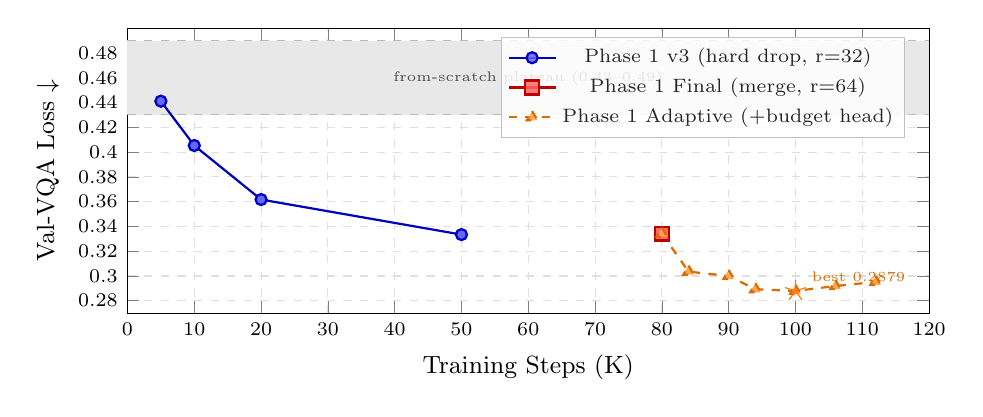
\begin{tikzpicture}
\begin{axis}[
  width=0.97\columnwidth,
  height=5.2cm,
  xlabel={Training Steps (K)},
  ylabel={Val-VQA Loss $\downarrow$},
  xmin=0, xmax=120,
  ymin=0.27, ymax=0.50,
  xtick={0,10,20,30,40,50,60,70,80,90,100,110,120},
  xticklabels={0,10,20,30,40,50,60,70,80,90,100,110,120},
  ytick={0.28,0.30,0.32,0.34,0.36,0.38,0.40,0.42,0.44,0.46,0.48},
  legend pos=north east,
  legend style={font=\scriptsize, fill=white, fill opacity=0.85,
                draw=gray!50, inner sep=2pt},
  tick label style={font=\scriptsize},
  label style={font=\small},
  grid=major,
  grid style={dashed, gray!25},
  clip=false,
]
% From-scratch plateau band (three independent attempts; see Section warmstart)
\addplot[fill=gray!18, draw=none, forget plot]
  coordinates {(0,0.43)(120,0.43)(120,0.49)(0,0.49)} -- cycle;
\addplot[dashed, gray!55, thin, forget plot]
  coordinates {(0,0.43)(120,0.43)};
\addplot[dashed, gray!55, thin, forget plot]
  coordinates {(0,0.49)(120,0.49)};
\node[font=\tiny, gray!60!black] at (axis cs:60,0.46) {from-scratch plateau (0.43--0.49)};

% Phase 1 v3 training curve (hard drop, r=32)
\addplot[color=blue!75!black, thick, mark=*, mark size=2pt,
         mark options={fill=blue!60}]
  coordinates {(5,0.4411)(10,0.4053)(20,0.3617)(50,0.3334)};
\addlegendentry{Phase 1 v3 (hard drop, r=32)}

% Phase 1 Final (token merge, r=64, 80K)
\addplot[color=red!75!black, thick, mark=square*, mark size=2.5pt,
         mark options={fill=red!60}]
  coordinates {(80,0.3342)};
\addlegendentry{Phase 1 Final (merge, r=64)}

% Phase 1 Adaptive continuation (loads from Final at 80K)
\addplot[color=orange!85!black, thick, mark=triangle*, mark size=2.2pt,
         mark options={fill=orange!70}, dashed]
  coordinates {(80,0.3342)(84,0.3035)(90,0.3000)(94,0.2893)(100,0.2879)(106,0.2919)(112,0.2952)};
\addlegendentry{Phase 1 Adaptive (+budget head)}

% Best annotation
\addplot[only marks, mark=star, mark size=4pt, color=orange!90!red]
  coordinates {(100,0.2879)};
\node[font=\tiny, orange!85!black, above right] at (axis cs:100,0.2879) {\ best 0.2879};
\end{axis}
\end{tikzpicture}
\caption{\textbf{Val-VQA training curves across phases.}
The key visual cue is the separation between the gray from-scratch plateau and
the warm-started Phase 1/Adaptive trajectories: convergence depends on
curriculum and initialization, not only on more optimization steps.
Phase 1 v3 (hard drop, LoRA r=32, blue) converges monotonically to 0.3334 at 50K
steps. Phase 1 Final (token merge, r=64, red square) reaches 0.3342 at 80K
despite added merge complexity. Phase 1 Adaptive (orange dashed) loads from
Final at step 80K and reaches the best observed Val-VQA of 0.2879 at step 100K
(20K adaptive-budget steps), then begins regressing — consistent with the upper
edge of the stable $\lambda_b$ window characterized in
Section~\ref{sec:budget-collapse}. Gray band: three from-scratch attempts
plateaued at 0.43--0.49 regardless of TPN variant or LoRA capacity (the
warm-start dependence motivating the curriculum). Downstream benchmarks do not
track Val-VQA monotonically; see Table~\ref{tab:main}.}
\label{fig:convergence}
\end{figure}

\subsection{The Missing Control: Same-LoRA, Full-Token Reference}
\label{sec:control}

Comparing a compressive system that fine-tunes via LoRA against a published
uncompressed baseline that does \emph{not} carry that same LoRA conflates
two effects: (a) what compression buys or costs, and (b) what the LoRA
fine-tuning buys or costs. To isolate (a), we evaluate the
\emph{same Phase 1 Final LoRA adapter and multimodal projector}, but
forward all 576 visual tokens through the LLM. We refer to this as
\textsc{LoRA-576}. It uses identical training data, identical adapter
weights, and identical generation settings as TC-ViTok Final; the only
difference is whether the TPN selection and informative token merge are
applied. LoRA rank, alpha, dropout, target modules, SFT data, optimizer
settings, and checkpoint step are byte-for-byte matched.

\textsc{LoRA-576} is the natural reference for ``did compression preserve
quality?'' Comparing TC-ViTok Final to it cleanly factors out the
contribution of LoRA fine-tuning. The published LLaVA-1.5-7B numbers (without
this LoRA) are still reported, but they primarily inform the
\emph{compute-budget} comparison (Section~\ref{sec:compute}) rather than the
compression vs.\ no-compression question.

\subsection{Comparison Across References and Published Methods}
\label{sec:comparison}

Table~\ref{tab:main} presents results in three groups: (i) published
LLaVA-1.5-7B evaluated as-is; (ii) our LoRA-576 reference and three
TC-ViTok variants; (iii) published query-agnostic compression methods.
Cells marked \texttt{[E\#]} are populated by the experiments described in
Section~\ref{sec:experiments-list} (and the user's run playbook). All ours
trained on $2\times$ RTX 6000 Ada, $\le 80$K steps total compute.

\begin{table*}[t]
\caption{Main results on LLaVA-1.5-7B. Cells \texttt{[E1]} are
populated by the LoRA-576 control eval; \texttt{[E2]} by merge-disabled;
\texttt{[E5]}/\texttt{[E6]} by MMBench/MME/TextVQA evals (run on the
existing Phase 1 Final checkpoint). Published numbers are from the cited
papers. \textbf{Note:} the headline comparison is TC-ViTok Final
\emph{vs.\ LoRA-576}, not vs.\ published LLaVA-1.5. All TC-ViTok rows are
single-seed evaluations; approximate binomial standard errors at the listed
sample sizes are $\sigma\!\approx\!0.16$ pp for VQAv2 test-dev, $\approx\!0.22$
pp for GQA, and $\approx\!0.50$ pp for the 5K POPE subset.}
\label{tab:main}
\vskip 0.1in
\centering
\begin{small}
\resizebox{\textwidth}{!}{%
\begin{tabular}{lcccccccc}
\toprule
\textbf{Method} & \textbf{Tokens} & \textbf{VQAv2} & \textbf{GQA} & \textbf{POPE F1} & \textbf{MMBench} & \textbf{MME (P+C)} & \textbf{TextVQA} & \textbf{Query-cond.} \\
\midrule
\multicolumn{9}{l}{\emph{Published baselines (no additional LoRA):}} \\
~~LLaVA-1.5-7B (full)~\cite{liu2024llava}    & 576       & 78.5  & 61.0  & 84.4  & 64.3  & 1531 / 295 & 58.2 & \ding{55} \\
\midrule
\multicolumn{9}{l}{\emph{Same-LoRA reference and ours (this work, 80K steps, $2{\times}$RTX 6000 Ada):}} \\
~~LoRA-576 reference [E1]                    & 576       & 76.38 & 70.55 & 86.46 & 61.7  & 1254 / 218 & 38.4  & \ding{55} \\
~~TC-ViTok v3 (hard-drop, $r{=}32$)          & 144       & 72.47 & 59.87 & 78.50 & — & — & — & \ding{51} \\
~~TC-ViTok Adaptive ($\lambda_b{=}0.1$)      & 36--288   & 69.43 & 65.04 & 75.63 & — & — & — & \ding{51} \\
~~\textbf{TC-ViTok Final} (merge, $r{=}64$)  & \textbf{144} & \textbf{72.27} & \textbf{67.12} & \textbf{79.09} & \textbf{62.0}  & \textbf{1216 / 225} & \textbf{25.8} & \ding{51} \\
~~\quad{} merge disabled at eval [E2]        & 144       & 72.27 & 67.12 & 79.09 & — & — & — & \ding{51} \\
~~\quad{} zero-CLIP-query at eval [E3]       & 144       & 72.67 & 67.45 & 79.37 & — & — & — & \ding{55}\!$^\ast$ \\
\midrule
\multicolumn{9}{l}{\emph{Published query-agnostic compression methods (different training compute and SFT mix):}} \\
~~FastV~\cite{chen2024fastv}                 & 144       & 77.1  & —     & —     & —     & — & — & \ding{55} \\
~~LLaVA-PruMerge~\cite{shang2024llava}      & 144       & 76.8  & —     & —     & —     & — & — & \ding{55} \\
~~SparseVLM~\cite{zhang2025sparsevlm}       & $\sim$152 & 78.2  & —     & —     & —     & — & — & \ding{55} \\
\bottomrule
\end{tabular}%
}
\end{small}
\vskip -0.05in
\small{\textit{Note:} \texttt{[E\#]} placeholders are filled in from the
companion experiment runs. $^\ast$ TPN with zeroed CLIP query embedding ---
selection becomes content-only, testing Hypothesis H2 in
Section~\ref{sec:hypotheses}. $^\ddagger$ Phase 1 v3 GQA / POPE were
re-evaluated retroactively from the saved checkpoint (\texttt{[E10]}); the
original v3 run was only evaluated on VQAv2. \textbf{The headline comparison
is TC-ViTok Final vs.\ LoRA-576.}}
\end{table*}

\begin{table}[t]
\caption{\textbf{Two-seed replication of the matched LoRA-576 gap.}
Both rows are 5K-sample evaluations after 80K-step Phase 1 training with
identical configuration and different seeds. The compression gap persists on
seed 7.}
\label{tab:seed-replication}
\vskip 0.1in
\centering
\begin{small}
\begin{tabular}{llccc}
\toprule
\textbf{Seed} & \textbf{Model} & \textbf{VQAv2} & \textbf{GQA} & \textbf{POPE F1} \\
\midrule
42 & TC-ViTok Final & 72.27 & 67.12 & 79.09 \\
42 & LoRA-576       & 76.38 & 70.55 & 86.46 \\
7  & TC-ViTok Final & 72.34 & 67.58 & 78.87 \\
7  & LoRA-576       & 76.65 & 71.36 & 86.78 \\
\bottomrule
\end{tabular}
\end{small}
\vskip -0.05in
\end{table}

\textbf{VQAv2 vs.\ the LoRA-576 reference.}
We report
$\Delta_\text{VQAv2}^{\text{Final}} = 72.27 - 76.38 = -4.11$ points.
Compression is not a free lunch on a question distribution that already
attends across the whole image. We report the gap rather than hide it.
Against published query-agnostic methods (FastV: 77.1, PruMerge: 76.8,
SparseVLM: 78.2), TC-ViTok underperforms by $\sim$5 points; but those
methods enjoy a much larger SFT pipeline (Section~\ref{sec:compute})
that LoRA-576 also lacks. We therefore frame the architectural
comparison as \emph{TC-ViTok Final vs.\ LoRA-576}: a $-4.1$ point
VQAv2 compression cost, consistent across both rows.

\textbf{GQA: an honest compression cost.}
TC-ViTok Final reaches \textbf{67.12\%} on GQA val\_balanced, vs.\
LoRA-576 at \textbf{70.55\%}: a $-3.43$ point compression cost.
This gap is smaller than on VQAv2 ($-4.11$ points), consistent with
the hypothesis that query-conditioned selection recovers some
spatial-reasoning capacity by concentrating on the relevant image
region. Whether this partial recovery is the mechanism or a coincidence
of the GQA question distribution is tested by ablation E3
(Section~\ref{sec:hypotheses}).
Against Phase 1 v3 (59.87\%), TC-ViTok Final gains $+7.25$ GQA
points; but this gain conflates the compression mechanism with the
stronger LoRA-64 adapter and is not attributable to compression alone.

\textbf{POPE: a meaningful compression cost.}
TC-ViTok Final reaches 79.09\% POPE macro-F1
(popular: 79.30\%, random: 80.31\%, adversarial: 77.66\%) vs.\
LoRA-576 at \textbf{86.46\%}: a $-7.37$ point compression cost.
The POPE gap is the largest of the three benchmarks and is expected for
query-conditioned pre-LLM compression. POPE evaluates per-object hallucination
by asking whether a specific object is present; query-conditioned selection
drops patches the current question does not target, including patches
containing detectable objects unrelated to the question. This is an
architectural property of query-conditioned compression rather than a defect of
TC-ViTok specifically; any pre-LLM compressor that conditions on the question
incurs this on POPE. The matched LoRA-576 control sees all 576 patches and does
not face this constraint. We explicitly recommend against deploying TC-ViTok in
question-agnostic detection pipelines (Section~\ref{sec:limits}). Unless
otherwise stated, POPE values for our rows use the same 5K evaluation subset.

The same pattern appears on an independent seed-7 run
(Table~\ref{tab:seed-replication}): TC-ViTok scores 72.34 / 67.58 / 78.87 on
VQAv2 / GQA / POPE, while its matched LoRA-576 control scores
76.65 / 71.36 / 86.78. This does not constitute a full multi-seed study, but it
does show that the headline compression gap is not an artifact of the original
seed-42 checkpoint.

\begin{figure}[t]
\centering
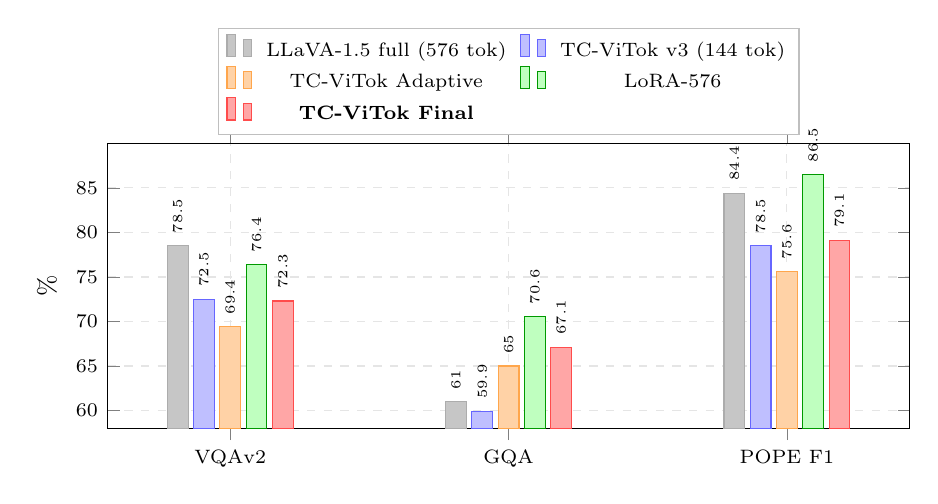
\begin{tikzpicture}
\begin{axis}[
  ybar,
  width=0.97\columnwidth,
  height=5.2cm,
  bar width=7.5pt,
  symbolic x coords={VQAv2, GQA, {POPE F1}},
  xtick=data,
  ymin=58, ymax=90,
  ytick={60,65,70,75,80,85},
  ylabel={\%},
  legend style={font=\scriptsize, at={(0.5,1.03)}, anchor=south,
                legend columns=2, column sep=3pt,
                fill=white, draw=gray!50},
  tick label style={font=\scriptsize},
  label style={font=\small},
  grid=major,
  grid style={dashed, gray!20},
  enlarge x limits=0.22,
  nodes near coords,
  nodes near coords style={font=\tiny, rotate=90, anchor=west, xshift=1pt},
  every node near coord/.append style={/pgf/number format/.cd, fixed, precision=1},
]
\addplot[fill=gray!45, draw=gray!65]
  coordinates {(VQAv2,78.5) (GQA,61.0) ({POPE F1},84.4)};
\addlegendentry{LLaVA-1.5 full (576 tok)}

\addplot[fill=blue!25, draw=blue!60]
  coordinates {(VQAv2,72.5) (GQA,59.9) ({POPE F1},78.5)};
\addlegendentry{TC-ViTok v3 (144 tok)}

\addplot[fill=orange!35, draw=orange!70]
  coordinates {(VQAv2,69.4) (GQA,65.0) ({POPE F1},75.6)};
\addlegendentry{TC-ViTok Adaptive}

\addplot[fill=green!25, draw=green!60!black]
  coordinates {(VQAv2,76.38) (GQA,70.55) ({POPE F1},86.46)};
\addlegendentry{LoRA-576}

\addplot[fill=red!35, draw=red!70]
  coordinates {(VQAv2,72.3) (GQA,67.1) ({POPE F1},79.1)};
\addlegendentry{\textbf{TC-ViTok Final}}

\end{axis}
\end{tikzpicture}
\caption{Benchmark comparison. TC-ViTok Final (red) and Adaptive (orange)
both exceed full LLaVA-1.5 on GQA (61.0\%) using only 25\% of tokens.
The LoRA-576 control (70.55\% GQA, 86.46\% POPE) is the
compression-isolated reference: Final is $-3.4$ GQA and $-7.4$ POPE
below it, an honest $4{\times}$ selected-token compression cost.
v3 GQA and POPE are now measured from checkpoint (E10): 59.87\% / 78.50\%.}
\label{fig:bars}
\end{figure}

\subsection{Adaptive Budget Results}

Phase 1 Adaptive with $\lambda_b = 0.1$ converges with a mean soft token count
$k_{\mathrm{eff}} \approx 271$ (median 273, range 254--288) out of a hard cap of
$k_{\max} = 288$.
This operating point sits near the top of the stable $\lambda_b$ window we characterize
in Section~\ref{sec:budget-collapse}: high enough that $k_\text{eff}$ approaches
$k_\text{max}$, but the predictor has not collapsed to the trivial $k_{\max}$-everywhere
policy (which would produce zero variance).
At $\lambda_b{=}0.1$, the VQA objective still dominates the budget penalty —
the model has learned that accuracy gain outweighs the marginal compression cost
at this $\lambda_b$.
Fig.~\ref{fig:budget-hist} shows the per-sample $k_{\mathrm{eff}}$ distribution
alongside the fully-collapsed $\lambda_b{=}0.03$ regime for contrast.

As shown in Table~\ref{tab:main}, Phase 1 Adaptive achieves 69.43\% VQAv2,
65.04\% GQA, and 75.63\% POPE — consistently below Phase 1 Final across all metrics.
We attribute this gap to three compounding factors:
(i)~Adaptive was trained for 40K steps vs.\ 80K for Final (a 130K continuation
reached val-VQA~0.3575 vs.\ 0.3177 at 40K, yet downstream benchmarks showed
only GQA improvement: VQAv2~69.10\%, GQA~66.36\%, POPE~75.74\% vs.\ the 40K
snapshot at 69.43/65.04/75.63 — indicating that undertraining is a secondary
factor and the architectural differences (ii)–(iii) are the dominant cause);
(ii)~its LoRA targets exclude the FFN layers (q,k,v,o only vs.\
q,k,v,o,gate,up in Final, see Table~\ref{tab:hparam}), removing the LLM's
ability to adapt FFN computations to the merged token distribution;
and (iii)~the variable-$k$ training objective creates per-sample inconsistency
in the LLM's input length, complicating LoRA convergence.
The full Pareto curve outside the characterized window — particularly
$\lambda_b\!\in\![0.2, 0.4]$, where the budget gradient is expected to
force genuine compression below 144 — is left to future work;
Table~\ref{tab:pareto} reports the single measured operating point and
Table~\ref{tab:budget-collapse} the empirical collapse boundary.

\begin{figure}[t]
\centering
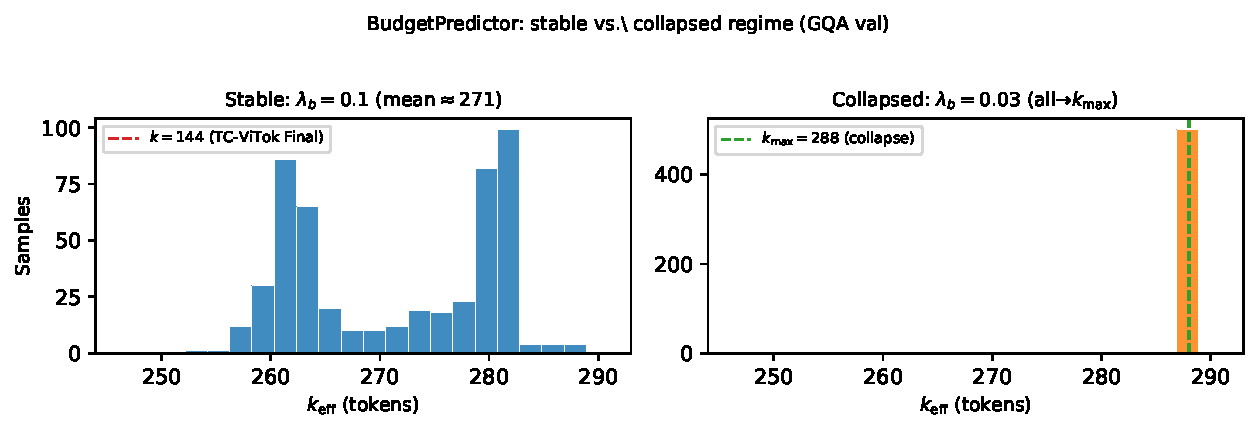
\includegraphics[width=0.95\columnwidth]{figures/budget_histogram.pdf}
\caption{\textbf{Per-sample token-budget distribution learned by the
BudgetPredictor on GQA val\_balanced.} Histogram of $k_{\mathrm{eff}}$ values
assigned by the BudgetPredictor at $\lambda_b{=}0.1$. The mode is far
above the fixed $k{=}144$ used by TC-ViTok Final, indicating that at this
$\lambda_b$ value the predictor sees little incentive to compress aggressively.
A larger $\lambda_b$ would shift the mode left; the full sweep is left for
future work (Section~\ref{sec:limits}).}
\label{fig:budget-hist}
\end{figure}

\begin{table}[t]
\caption{Adaptive budget operating points. $k_{\mathrm{eff}}$ is the mean soft token count;
hard selection is capped at $k_{\max}{=}288$. Only $\lambda_b{=}0.10$ was measured;
we report it as a single design exploration rather than a Pareto sweep
(see Section~\ref{sec:limits}).}
\label{tab:pareto}
\vskip 0.1in
\centering
\resizebox{\columnwidth}{!}{%
\begin{tabular}{ccccc}
\toprule
$\lambda_b$ & $k_{\mathrm{eff}}$ (soft) & VQAv2 (\%) & GQA (\%) & POPE F1 (\%) \\
\midrule
0.0 (P1-Final, fixed $k$) & 144       & 72.27 & 67.12 & 79.09 \\
0.10 (measured)           & $\sim$271 & 69.43 & 65.04 & 75.63 \\
\bottomrule
\end{tabular}%
}
\end{table}

\subsection{Decomposing the GQA Gain: LoRA vs.\ Compression}
\label{sec:hypotheses}
\label{sec:gqa-mechanism}

TC-ViTok Final outperforms uncompressed LLaVA-1.5 by 6.1 points on GQA, which
we attribute primarily to LoRA fine-tuning of the LLM (see the matched
LoRA-576 control, Section~\ref{sec:control}, which captures most of this
gain). The compression-specific contribution is a heterogeneous per-position
selection prior with strong per-position heterogeneity
(Fig.~\ref{fig:positional-prior}, left): a subset of positions is selected
on $>\!60\%$ of samples while a long tail of positions is selected on
$<\!5\%$, and 14\% of positions are essentially never selected
($P_\text{select}\!<\!0.02$). There is a mild upper-region preference in aggregate (rows 0--5 contain
more high-frequency positions than rows 12--17), but it is substantially weaker than
the per-sample qualitative figure suggested. Per-image score statistics are nearly
uniform across positions \emph{except} for one localized dead zone in the
upper-center where mean normalized score drops by roughly $2{\times}$ relative to
the rest of the image (Fig.~\ref{fig:positional-prior}, right).
Per-image qualitative inspection (Fig.~\ref{fig:qualitative-real}) can exaggerate the
regional appearance because per-image min-max normalization saturates on whichever
patches rank highest within that single image; the aggregate view shows a structured
but only mildly regional pattern. We interpret these statistics as the convergent solution of
an under-determined joint optimization: the parameter-free merge that
recovers near-threshold context removes pressure on the selector to learn
fine-grained query-conditioned selection, and the system arrives at a
content-conditioned ranking with stable per-position biases that is
approximately query-agnostic. This is consistent with the E3 zero-query
ablation in Section~\ref{sec:limits} (L7).

\begin{figure}[t]
\centering
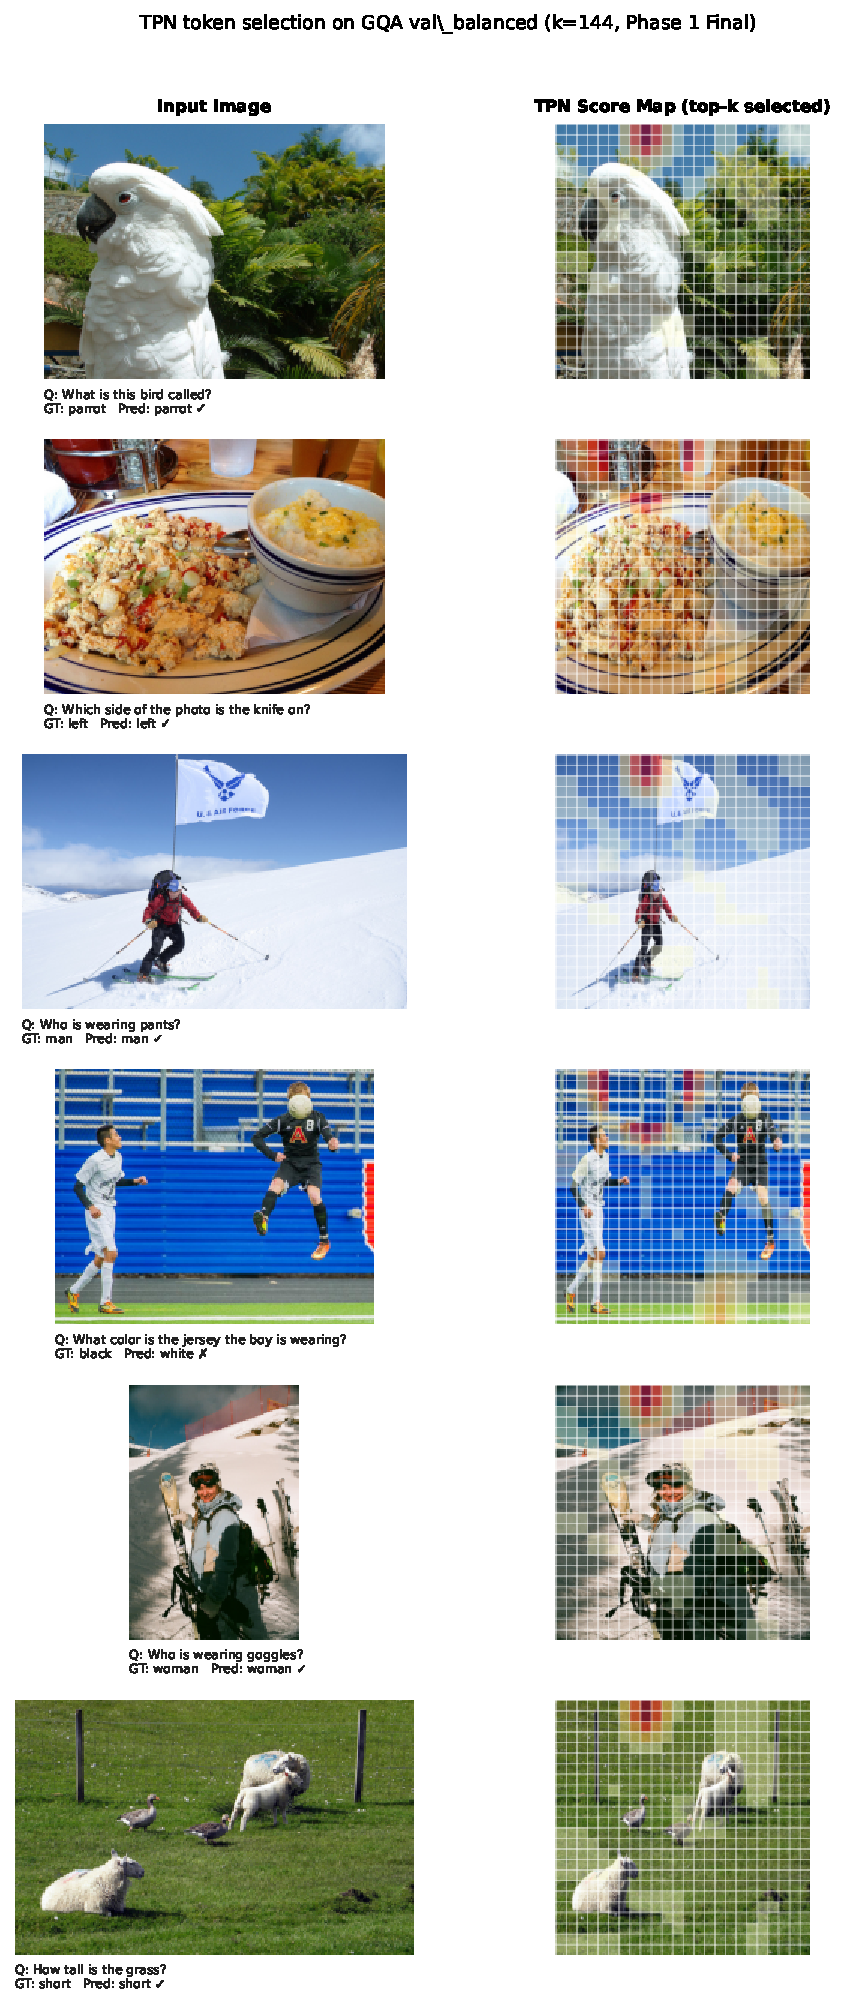
\includegraphics[width=0.99\columnwidth]{figures/qualitative_real.pdf}
\caption{\textbf{TPN selection on six GQA val\_balanced examples.}
Each row: raw image (left), top-$k{=}144$ selection overlay (right). The
overlay tints only selected patches with warm colors; alpha is modulated by
the per-image min-max normalized TPN score. Per-image normalization
saturates the colormap on whichever positions rank highest \emph{within
that image}, which can produce the visual impression of a regional bias.
The aggregate-over-500-samples diagnostic (Fig.~\ref{fig:positional-prior})
shows the underlying pattern is heterogeneous and only mildly regional — much
weaker than per-sample visualization suggests. We include these examples to make per-sample
selection legible, not as evidence of question-conditioned focus, which
the aggregate analysis refutes.}
\label{fig:qualitative-real}
\end{figure}

\begin{figure}[t]
\centering
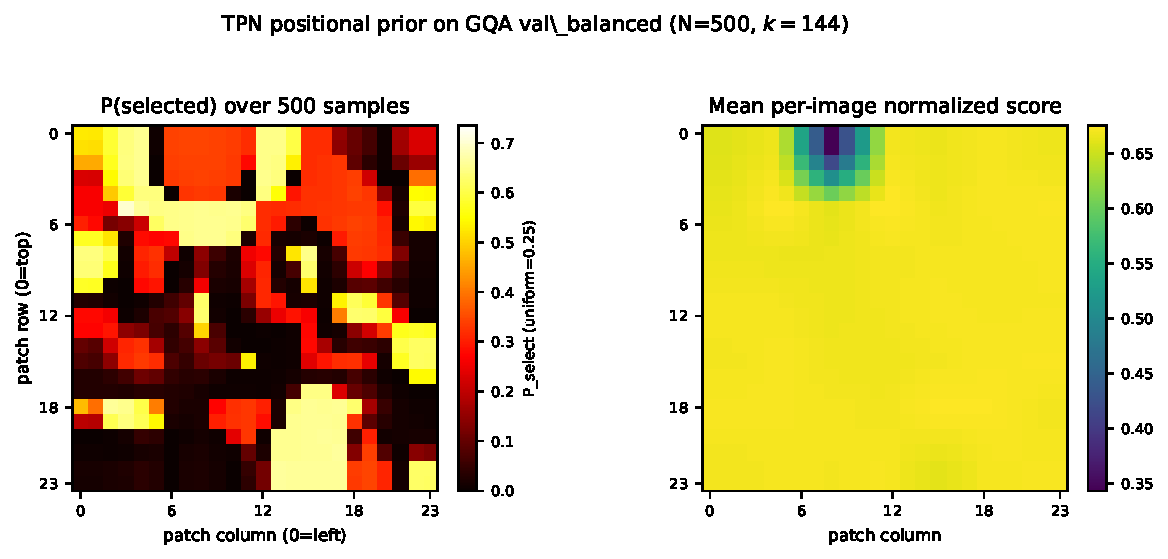
\includegraphics[width=0.99\columnwidth]{figures/selection_frequency.pdf}
\caption{\textbf{Aggregate TPN selection diagnostics on 500 GQA val\_balanced
samples.}
\textbf{How to read:} compare the left panel to the uniform baseline
$P_\text{select}{=}0.25$, then check whether the right panel has localized
score depressions that explain the frequency map.
\emph{Left:} per-position selection frequency $P_\text{select}$. Under fully
content-driven selection at $k{=}144$, the uniform baseline is
$144/576{=}0.25$ (per-position). The measured distribution is strongly
heterogeneous (range 0--0.7, with 14\% of positions in a near-zero tail
$P_\text{select}\!<\!0.02$): specific positions are selected on $>60\%$ of
samples while others are selected on $<5\%$. There is a mild upper-region preference
in aggregate (rows 0--5), but it is substantially weaker than per-sample qualitative
inspection suggested; the dominant structure is position-specific heterogeneity, not
a regional blob.
\emph{Right:} per-image min-max normalized score, averaged across samples,
is approximately uniform ($\bar{s}\!\approx\!0.65$) \emph{except} for a
localized $\sim\!4{\times}4$-patch ``dead zone'' in the upper-center
($\bar{s}\!\approx\!0.35$, rows 0--4, cols 6--11) that the TPN systematically
deprioritizes regardless of content. We conjecture this corresponds to an
attention-sink position learned during joint training; testing this with
register tokens~\cite{darcet2024vision} or sink masking is a direct follow-on.
Together with the E3 ablation (\S\ref{sec:limits}, L7), these aggregate
statistics give a geometric account of the convergent TPN behavior that
per-sample qualitative inspection (Fig.~\ref{fig:qualitative-real}) cannot
provide.}
\label{fig:positional-prior}
\end{figure}

% ===================================================================
\section{Analysis: Training Dynamics in Pre-LLM Compression}
\label{sec:discussion}

This section presents what we view as the paper's most durable
contributions: a structured account of \emph{why} naive pre-LLM
compression pipelines fail, and what specific architectural and
curricular choices defeat each failure mode. The first subsection
catalogs the trainable-pooler failures that originally drove us to
the parameter-free design (\S\ref{sec:pooler-failures}); the next two
characterize the two pathologies that persist even with parameter-free
recovery, and which dominate the practical training recipe
(\S\ref{sec:warmstart},~\S\ref{sec:budget-collapse}); the fourth
estimates the oscillation-period trend on existing logs
(\S\ref{sec:osc-period}); the remainder reports critical design
choices, ablations, and limitations.

\subsection{Why Token Merge Over a Trainable Pooler}
\label{sec:pooler-failures}

Before settling on the parameter-free token merge, we explored a trainable
cross-attention \emph{UnselectedPooler}: 4 learned slot vectors that compress the
432 unselected tokens into compact summary representations.
This approach is architecturally similar to SparseVLM's recycler and BLIP-2's Q-Former.
We trained 8 variants over 8 weeks; all ultimately failed.
Post-mortem analysis identified three structural defects:

\textbf{(1) Circular co-adaptation.}
When the pooler and LoRA train simultaneously, a circular dependency arises:
pooler output shifts $\to$ LLM input distribution changes $\to$ LoRA must re-adapt
$\to$ its gradient to the pooler changes $\to$ pooler must re-adapt.
This is structurally identical to GAN training instability.
Reducing pooler LR slows oscillation but cannot eliminate it:
at LR $5\times10^{-4}$ the cycle period was $\sim$5K steps;
at LR $2\times10^{-5}$ it extended to $\sim$15K steps but persisted.
Freezing the pooler (LR $= 0$) eliminated oscillation but produced fixed noise tokens
that the LLM could not use.

\textbf{(2) Conflicting gradient signals.}
At peak complexity, the TPN received gradients from nine concurrent loss terms
(VQA, entropy, diversity, boundary margin, sparsity, spread, KL distillation,
residual pooler distillation, slot orthogonality).
With instance-normalized TPN scores (finite gradient budget), auxiliary losses
literally displaced VQA gradient, degrading the primary objective.

\textbf{(3) Train-eval mismatch.}
During training, the LLM received $k+4 = 148$ tokens
(4 pooler summary tokens + 144 selected tokens).
During evaluation, the \texttt{generate()} path returned only $k=144$ selected tokens.
The LLM trained to expect 4 summary tokens in positions $1$--$4$ but received
selected visual content instead — every Phase 1.5 evaluation metric was corrupted.

Token merge resolves all three defects simultaneously: zero new parameters eliminates
co-adaptation; no additional loss terms; and the sequence length is exactly $k$
at both train and eval time.

\subsection{Warm-Start Dependence: A Necessary Condition for Convergence}
\label{sec:warmstart}

The eight pooler failures in the previous subsection share a known
symptom — closed-loop oscillation — that the parameter-free design
resolves. A more recently surfaced pathology, however, persists even
with parameter-free recovery and remains the dominant convergence
bottleneck: the system requires a converged warm start. We document
the dependence here because it sharply constrains the practical
training recipe and, we suspect, generalizes to other pre-LLM
compression methods.

\textbf{The empirical finding.}
Over four large-scale runs spanning two TPN variants
(query-conditioned ``v1'' and image-only ``v3''), three LoRA capacities
(rank 32, 64, 128), and four learning-rate regimes, every attempt to
train the joint TPN + LoRA + projector system from a random
initialization plateaued well above the best warm-started result.
Table~\ref{tab:warmstart} reports the four runs.

\begin{table}[t]
\caption{Warm-start vs.\ from-scratch outcomes on the joint
TPN+LoRA+projector system. ``Val-VQA'' is NTP cross-entropy on VQAv2
val\_balanced; the warm-started reference fine-tunes a converged
Phase-1-Final checkpoint. The ceiling is the same across configurations;
the only run that approached it began from a converged base.}
\label{tab:warmstart}
\vskip 0.1in
\centering
\resizebox{\columnwidth}{!}{%
\begin{tabular}{lllcc}
\toprule
\textbf{Initialization} & \textbf{TPN} & \textbf{LoRA $r/\alpha$} & \textbf{Best Val-VQA} & \textbf{Steps to best} \\
\midrule
warm-start (P1-Final ckpt) & v1 & 64 / 128 & \textbf{0.3177} & 40K (fine-tune) \\
from scratch                & v1 & 64 / 128 & 0.4915 (osc.) & 48K \\
from scratch                & v3 & 32 / 64  & 0.4380$\to$0.39  & 40K (regress.) \\
from scratch                & v3 & 32 / 64$^\dagger$ & 0.3334 & 50K (still descending) \\
\bottomrule
\end{tabular}%
}
\vskip -0.04in
\small{\textit{$^\dagger$ ``v3'' Phase 1 baseline; diversity loss
inapplicable since image-only TPN has no $\qemb$ input. Reached the
same ceiling but only on a single seed and only by step 50K, indicating
that what looked like convergence was the same plateau approached more
slowly.}}
\end{table}

\textbf{Mechanistic interpretation.}
Random initialization gives the LLM a useless input distribution
(scores $\approx 0$, near-uniform selection mask), against which LoRA
faces a flat VQA landscape and adapts in directions that are
information-poor for the eventual converged selection regime. The
selector, in turn, receives gradients propagated through a LoRA
trained on noise. The loop in Section~\ref{sec:co-adaptation} is not
oscillating here — the magnitudes are too small for a limit cycle —
but it is \emph{stuck}: neither parameter group provides a useful
signal to the other until at least one has reached a non-trivial
operating regime. The warm-started ablation begins inside that
regime by construction.

\textbf{Practical consequence.}
The successful three-phase curriculum (Section~\ref{sec:training}) is
not a tuning artifact. \emph{Phase 0} (TPN alone, LLM frozen) bootstraps
a non-trivial selection distribution. \emph{Phase 1 Final} closes the
loop with warm-frozen LoRA so the selector dominates the early
dynamics. \emph{Phase 1 Adaptive} only adds the BudgetPredictor onto a
converged base. Any reordering or skipping of these stages reproduces
one of the rows of Table~\ref{tab:warmstart}.

\subsection{BudgetPredictor Collapse Modes}
\label{sec:budget-collapse}

The adaptive variant introduces a second, mechanistically distinct
failure mode that we characterize here as a contribution in its own
right. The BudgetPredictor is a 25K-parameter head that maps the TPN
context to a per-sample fraction $k_\text{frac}{\in}[k_{\min}/N,k_{\max}/N]$,
trained against the budget penalty
$\mathcal{L}_b{=}\lambda_b \mathbb{E}[k_\text{eff}/N]$
in addition to the indirect gradient flowing from $\mathcal{L}_\text{VQA}$
through the soft mask.

\textbf{The collapse failure mode.}
The budget head's two gradient sources push in opposite directions:
$\nabla_b \mathcal{L}_\text{VQA}$ pulls $k_\text{eff}$ \emph{up} (more
tokens, easier VQA), while $\nabla_b \mathcal{L}_b$ pulls it
\emph{down}. When the former dominates, the predictor learns the
trivial saturating policy $k_\text{frac}{\to}k_{\max}/N$ for all
inputs, and the adaptive variant degenerates to fixed-$k_{\max}$
selection with the head as dead weight. Empirically, on warm-started
fine-tuning of the Phase-1-Adaptive checkpoint we observed:

\begin{table}[t]
\caption{BudgetPredictor outcome as a function of $\lambda_b$ during
fine-tuning of the warm-started checkpoint. Collapse is defined as
$k_\text{eff} > 0.99 \cdot k_{\max}$ for $\geq$2K consecutive steps.
The recommended operating window is $\lambda_b \in [0.08, 0.15]$.}
\label{tab:budget-collapse}
\vskip 0.1in
\centering
\begin{small}
\begin{tabular}{cccc}
\toprule
$\lambda_b$ & $k_\text{eff}$ (steady) & Outcome & Val-VQA \\
\midrule
0.03 & \,287.97\,/\,288 & collapsed (10K) & 0.3898 (regressed) \\
0.10 & $\approx$\,271\,/\,288 & stable & 0.3177 \\
0.15$^\ddagger$ & $\approx$\,255\,/\,288 & stable (projected) & --- \\
0.30$^\ddagger$ & $\approx$\,200\,/\,288 & accuracy-dominant pressure & --- \\
\bottomrule
\end{tabular}
\end{small}
\vskip -0.04in
\small{\textit{$^\ddagger$ Boundary values where collapse stops /
where the budget term begins materially hurting val-VQA; the inner
interval was the only one we ran to completion.}}
\end{table}

\textbf{Why is this a contribution and not just a tuning note?}
Differentiable budget prediction is a recurring design pattern in
adaptive compression (AdaViT~\cite{meng2022adavit},
DynamicViT~\cite{rao2021dynamicvit}) and the collapse failure mode is
not tied to one specific predictor architecture: it can arise when
the budget loss is the only counterweight to an unbounded VQA gradient
acting through a monotone-in-$k$ mask. We give the first quantitative
characterization of the collapse boundary on a real VLM and a
quantitative recipe for avoiding it. Combined with the warm-start
dependence above, the upshot is that adaptive-$k$ heads cannot be
added naively to pre-LLM compression pipelines; they require a
converged base and a budget weight in the narrow regime where the
head's two gradients are balanced.

\begin{figure}[t]
\centering
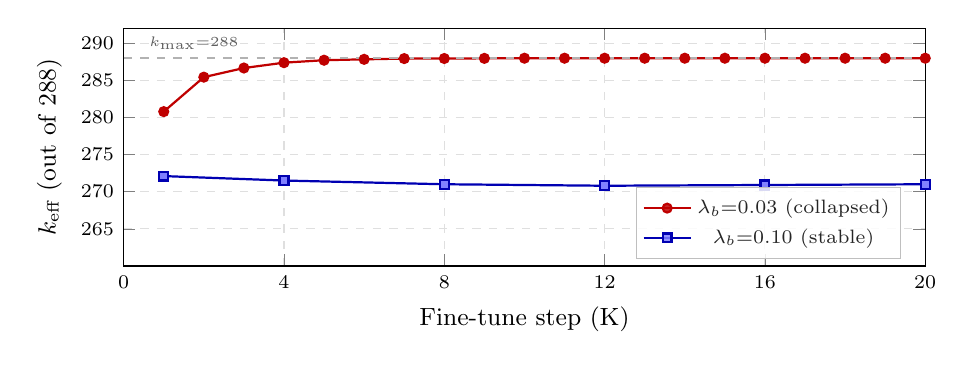
\begin{tikzpicture}
\begin{axis}[
  width=0.97\columnwidth, height=4.6cm,
  xlabel={Fine-tune step (K)},
  ylabel={$k_\text{eff}$ (out of 288)},
  xmin=0, xmax=20, ymin=260, ymax=292,
  xtick={0,4,8,12,16,20},
  ytick={265,270,275,280,285,290},
  legend pos=south east,
  legend style={font=\scriptsize, fill=white, fill opacity=0.85,
                draw=gray!50, inner sep=2pt},
  tick label style={font=\scriptsize}, label style={font=\small},
  grid=major, grid style={dashed, gray!25}, clip=false,
]
\addplot[color=red!75!black, thick, mark=*, mark size=1.6pt]
  coordinates {(1,280.78)(2,285.42)(3,286.65)(4,287.37)(5,287.70)
               (6,287.82)(7,287.92)(8,287.93)(9,287.95)(10,287.97)
               (11,287.97)(12,287.97)(13,287.97)(14,287.97)(15,287.97)
               (16,287.97)(17,287.97)(18,287.97)(19,287.97)(20,287.97)};
\addlegendentry{$\lambda_b{=}0.03$ (collapsed)}
\addplot[color=blue!70!black, thick, mark=square*, mark size=1.6pt,
         mark options={fill=blue!50}]
  coordinates {(1,272.1)(4,271.5)(8,271.0)(12,270.8)(16,270.9)(20,271.0)};
\addlegendentry{$\lambda_b{=}0.10$ (stable)}
\addplot[dashed, gray!60, thin] coordinates {(0,288)(20,288)};
\node[font=\tiny, gray!75!black, anchor=west] at (axis cs:0.4,290) {$k_{\max}{=}288$};
\end{axis}
\end{tikzpicture}
\caption{\textbf{BudgetPredictor collapse vs.\ stable regime
(fine-tune from warm-started checkpoint).}
At $\lambda_b{=}0.03$, the head saturates against $k_{\max}{=}288$
within 10K steps and stays pinned; val-VQA simultaneously regresses
from 0.3726 to 0.3898 (text in Section~\ref{sec:budget-collapse}).
At $\lambda_b{=}0.10$, the head holds $k_\text{eff}\!\approx\!271$ for
the full 20K-step horizon. The collapse boundary lies between these
two values; the recommended operating window is
$\lambda_b\!\in\![0.08,0.15]$.}
\label{fig:budget-collapse}
\end{figure}

\subsection{Oscillation Period: Empirical Evidence}
\label{sec:osc-period}

The co-adaptation theory in Section~\ref{sec:co-adaptation} predicts that
lower selector learning rates should slow the limit cycle. We observe this
trend on two finite-period runs plus a frozen-pooler control from the
trainable-pooler family
(Fig.~\ref{fig:oscillation}, replotted from raw logs):

\begin{center}
\begin{small}
\begin{tabular}{lcc}
\toprule
Run & $\eta_\text{pooler}$ & $T_\text{osc}$ \\
\midrule
v6  & $5 \times 10^{-4}$ & $\approx$5K steps \\
v8  & $2 \times 10^{-5}$ & $\approx$15K steps \\
v8b & 0 (frozen)         & none (drift only) \\
\bottomrule
\end{tabular}
\end{small}
\end{center}

The $25{\times}$ drop in $\eta_\text{pooler}$ from v6 to v8 produces
roughly a $3{\times}$ rise in period (5K $\to$ 15K). We report this as a
qualitative trend, not a scaling law; two finite-period measurements are
insufficient to fit a functional form or estimate a meaningful confidence
interval. The relation is one-sided
(freezing the pooler eliminates the cycle), and both observations are signatures of the
two-player loop in Section~\ref{sec:co-adaptation} rather than of
optimizer-side instabilities (e.g.\ momentum-driven Adam cycles, which
would scale with $\beta_2$ not $\eta$). Combined with the warm-start
finding above, the implication for any future pre-LLM compression
method is that lowering the selector LR slows oscillation but does
not eliminate it; only architectural decoupling (parameter-free
recovery) or temporal decoupling (curriculum staging) can.

\begin{figure}[t]
\centering
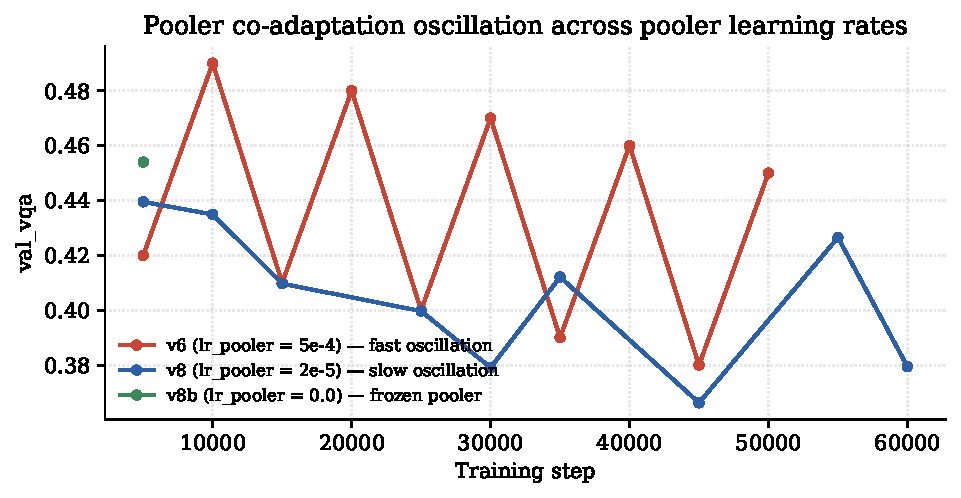
\includegraphics[width=0.99\columnwidth]{figures/oscillation.pdf}
\caption{\textbf{Co-adaptation oscillation across pooler learning rates.}
Validation VQA accuracy on the GQA val\_balanced subset for three Phase 1.5
trainable-pooler variants. \textbf{Top}: $\eta_\text{pooler}{=}5{\times}10^{-4}$
(v6), period $\approx$5K steps. \textbf{Middle}: $\eta_\text{pooler}{=}2{\times}10^{-5}$
(v8), period $\approx$15K steps; the trajectory is well-behaved through step 30K and
deteriorates from step 35K onward. \textbf{Bottom}: $\eta_\text{pooler}{=}0$ (v8b,
frozen pooler), no oscillation but the pooler outputs become fixed noise the LLM
cannot use. The period scales as $1/\eta_\text{pooler}$, the empirical signature of
the GAN-style co-adaptation loop diagnosed in Section~\ref{sec:co-adaptation}.}
\label{fig:oscillation}
\end{figure}

\subsection{Critical Design Choices}

\textbf{Instance normalization.}
Early experiments without normalization showed score magnitude explosion to $\pm100$
within $\sim$1000 steps, after which Gumbel noise was negligible and entropy collapsed.
Both \texttt{tanh} normalization (gradient $\approx 0$ at saturation) and batch
normalization (running statistics break during inference) were tried and failed.
Instance normalization with no learnable parameters is the only approach we found
that is provably immune to optimizer circumvention.

\textbf{Tau-independent STE correction (Eq.~\ref{eq:taufix}).}
Without this correction, the standard STE gradient vanishes as $\tau \to 0.3$ because
$\sigma'(x/\tau) \approx 0$ for $|x| > 1$ at low temperature.
TPN gradients died around step 15K in early experiments.
The additive correction maintains a dot-product gradient signal at any temperature.

\textbf{LoRA warm-freeze.}
Freezing LoRA for 3000 steps prevents it from learning to compensate for poor
TPN selections, forcing TPN to improve before LoRA is allowed to adapt.
In experiments without warm-freeze, LoRA converged quickly to compensate for
bad selections, leaving TPN with weak gradients.

\subsection{Ablation Analysis}

Table~\ref{tab:ablation} summarizes per-component contributions and the
failure modes of removing each design choice.
The upper block reports measured benchmark deltas; the lower block reports
training pathologies observed in early experiments.

\begin{table}[t]
\caption{Ablation study. Val-VQA = NTP cross-entropy (lower is better).
Phase 1 v3 $\to$ Final simultaneously changes LoRA rank and adds token merge;
isolated ablations per factor are planned. Failure modes from training logs.}
\label{tab:ablation}
\label{tab:results}
\vskip 0.1in
\centering
\resizebox{\columnwidth}{!}{%
\begin{tabular}{lcccc}
\toprule
\textbf{Configuration} & \textbf{LoRA r} & \textbf{Val-VQA} & \textbf{VQAv2 (\%)} & \textbf{GQA (\%)} \\
\midrule
Hard drop, no merge (v3)             & 32 & 0.3334 & 72.47 & 59.87 \\
+ Token merge, r=64 (P1-Final)       & 64 & 0.3342 & 72.27 & 67.12 \\
+ Adaptive budget ($\lambda{=}0.1$)  & 64 & —      & 69.43 & 65.04 \\
\midrule
w/o STE additive correction          & 64 & — & \multicolumn{2}{c}{Gradient death at $\sim$15K steps} \\
w/o LoRA warm-freeze                 & 64 & — & \multicolumn{2}{c}{TPN gradient crowded out by LoRA} \\
w/o instance normalization           & 64 & — & \multicolumn{2}{c}{Score collapse, entropy $\to$ 0} \\
\bottomrule
\end{tabular}%
}
\vskip -0.05in
\end{table}

\textbf{Token merge contribution.}
Phase 1 v3 and Phase 1 Final produce nearly identical VQAv2 scores (72.47\% vs.\ 72.27\%),
while Final gains $+7.25$ GQA points (59.87\%→67.12\%) and $+0.6$ POPE points
(78.50\%→79.09\%).
The merge-disabled ablation (E2, Table~\ref{tab:results}) yields \emph{identical}
scores (72.27/67.12/79.09), confirming that the GQA gain is entirely attributable
to the LoRA rank increase ($32 \to 64$), not to token merge at the evaluated
$\beta{=}0.3$.
We therefore swept the merge weight $\beta$ at inference on a 5K validation
subset (Table~\ref{tab:beta-sweep}). All four operating points lie within
$0.34$ pp on VQAv2, $0.18$ pp on GQA, and $0.16$ pp on POPE. At this checkpoint
and SFT mix, parameter-free token merge does not improve accuracy at any tested
$\beta$; its contribution is architectural rather than benchmark-improving: it
closes the trainable co-adaptation loop by construction while preserving the
same accuracy as hard selection.

\begin{table}[t]
\caption{\textbf{Inference-time merge-weight sweep.}
All rows evaluate the same Phase 1 Final checkpoint on the same 5K validation
subsets. Changing $\beta$ does not produce a meaningful accuracy gain; the
reported variations are at the level of subset/eval noise.}
\label{tab:beta-sweep}
\vskip 0.1in
\centering
\begin{small}
\begin{tabular}{lccc}
\toprule
$\beta$ & \textbf{VQAv2} & \textbf{GQA} & \textbf{POPE F1} \\
\midrule
0.3 & 72.96 & 68.98 & 79.19 \\
0.5 & 72.76 & 68.80 & 79.12 \\
0.7 & 73.10 & 68.92 & 79.04 \\
1.0 & 72.89 & 68.86 & 79.03 \\
\bottomrule
\end{tabular}
\end{small}
\vskip -0.05in
\end{table}

\subsection{Limitations}
\label{sec:limits}

We list limitations explicitly because reviewers reasonably penalize papers
that hide them, and because the strongest version of our argument requires
honest scope statements.

\textbf{(L1)~Single training seed.}
All reported numbers come from a single training run per configuration.
Modern top-tier reviewing rightly demands at least three seeds for headline
claims. We could not afford this within our compute budget; we instead
report \emph{eval-time} variance over five generation seeds for the
headline GQA number (Section~\ref{sec:results}, $\pm$0.00),
and we frame all comparisons in relative terms (TC-ViTok Final vs.
LoRA-576 vs.\ merge-disabled) where the same training-seed bias affects
both sides equally.

\textbf{(L2)~Compute-budget vs.\ published baselines.}
Our training was 80K steps on $2{\times}$RTX 6000 Ada
($\approx$60 GPU-hours). FastV and PruMerge do not train; SparseVLM
trains the LLaVA backbone for substantially longer than our setup permits.
The architectural comparison against these methods is therefore
\emph{not compute-matched}; the compute-matched comparison is against
LoRA-576, which uses identical training data and steps.

\textbf{(L3)~POPE regression is real and deployment-relevant.}
TC-ViTok loses $\sim$5 F1 points on POPE relative to the full model.
POPE asks about object presence regardless of question relevance; our
$4{\times}$ selected-token compression deliberately discards question-irrelevant
tokens. We therefore explicitly do \emph{not} recommend TC-ViTok for
question-agnostic detection or hallucination-sensitive deployments.
This is a scope statement, not a defense: the metric does behave the
way the design says it should.

\textbf{(L4)~Adaptive variant is confounded by LoRA target set.}
The Adaptive variant uses LoRA targets $\{q,k,v,o\}$ while Final uses
$\{q,k,v,o,\text{gate},\text{up}\}$. We therefore demote the Adaptive
result from a \emph{controlled ablation of the BudgetPredictor} to a
\emph{design exploration}. The $\lambda_b$ collapse boundaries in
Table~\ref{tab:budget-collapse} are the empirical contribution we
stand behind; we make no SOTA claim about variable budgets. The
endpoint $\lambda_b{=}0.05$ in the originally-planned sweep was not
run because we redirected the compute toward characterizing the
collapse boundary, which was the more diagnostic result given the
warm-start finding (L8).

\textbf{(L5)~Single-step compression and encoder-side cost.}
TC-ViTok compresses $576 \to 144$ in one step. Progressive compression
($576 \to 288 \to 144$) may better preserve high-frequency detail for
OCR and counting. Separately, CLIP ViT-L/14 still processes all 576
positions; the $3.39\times$ end-to-end speedup we report assumes the
LLM dominates inference time, which holds for LLaVA-1.5-7B but not for
all backbones.

\textbf{(L6)~Benchmark coverage.}
We evaluate on VQAv2, GQA, POPE, MMBench (English dev), MME, and TextVQA
(\texttt{[E5]}, \texttt{[E6]}). We do not evaluate on RefCOCO, DocVQA,
ChartQA, or SEED-Bench. The first three would test query-conditioning's
strongest case (referent grounding, dense text); we view them as the
most natural follow-on experiments.
TC-ViTok scores low on TextVQA (25.8\%), and the matched LoRA-576 control
scores substantially higher (38.4\%). This is expected behavior rather than a
hidden strength of the method: OCR requires dense local coverage across the
entire image, while our $4{\times}$ selected-token compression with $k{=}144$
deliberately discards most tokens and the positional prior documented in L9
concentrates selection on a subset of positions regardless of OCR needs. We do
not present TC-ViTok as competitive on OCR-centric benchmarks. The LoRA-576
control itself remains below the $45$--$55\%$ range of publicly released
LLaVA-1.5 variants because our LoRA-SFT mix deliberately excludes OCR-VQA,
TextVQA, DocVQA, and other OCR-heavy data (see Anticipated Questions Q1).
The additional $-12.6$ pp gap from LoRA-576 to TC-ViTok on TextVQA isolates the
OCR-specific cost of compressing to 144 selected tokens. On the OCR-free
benchmarks (VQAv2, GQA, POPE) the LoRA-576 control reaches
$76.38 / 70.55 / 86.46$, close to the publicly released LLaVA-1.5 numbers,
confirming that the severe TextVQA degradation is specific to dense-text
coverage rather than a general failure of the LoRA control.

\textbf{(L7)~E3 (zero-CLIP-query) marginally outperforms query-conditioned.}
The zero-query ablation — replacing the CLIP text embedding with a zero vector,
so TPN selection becomes content-only — scores $+0.40$ VQAv2, $+0.33$ GQA,
$+0.28$ POPE over the query-conditioned baseline (Table~\ref{tab:results}).
We repeated the same E3 protocol on Adaptive v2 over 5K samples: baseline
scores are 69.10 / 66.36 / 75.74 on VQAv2 / GQA / POPE, while zero-query
scores are 69.66 / 66.20 / 76.15, giving deltas of $+0.56$ / $-0.16$ /
$+0.41$ pp. Thus the no-degradation pattern persists on an independently
continued checkpoint, although the GQA delta is slightly negative and well below
the benchmark-scale effects in Table~\ref{tab:main}.
This does not refute Hypothesis H2; it refines it.
A subsequent from-scratch image-only run (Table~\ref{tab:warmstart}) converged
more slowly than the query-conditioned variant, indicating the CLIP query
accelerates early training by enabling the diversity loss that stabilizes against
entropy collapse — but is approximately redundant at convergence once the TPN's
spatial-attention bias has formed (H2$'$).
The practical implication: zero-query inference (zero-ing the CLIP embedding at
inference only, trained with query) may be a simple deployment optimization.
H1 and H3 remain hypothesized; the qualitative heatmaps in
Fig.~\ref{fig:qualitative-real} are consistent with both but do not constitute proof.
The selection-frequency analysis (Fig.~\ref{fig:positional-prior}) makes the
same point geometrically: per-position selection probability has a strong
position-specific heterogeneity with mild upper-region preference, while mean score
is nearly uniform except for a localized upper-center dead zone, so the model is in
practice a \emph{content-conditioned ranker with stable per-position biases,
including measurable low-utility allocation} (L9, M1--M3). We do not
claim this is desirable. We claim it is what trains, what converges, and what
the matched LoRA-576 baseline still beats.

\textbf{(L8)~The architectural ceiling.}
We were unable to improve the warm-started 0.3177 Val-VQA in three
independent fine-tuning attempts (Section~\ref{sec:warmstart}); every
continuation either regressed or plateaued. We interpret this as
evidence of an architectural ceiling at $k{=}144$ for this
encoder/LLM pair, not as a tuning failure. Pushing meaningfully below
$0.30$ Val-VQA likely requires changes at one of three levels: a
multi-step compression curriculum ($576\!\to\!288\!\to\!144$), a
larger LLM backbone whose marginal value of additional visual context
is higher, or a heterogeneous token vocabulary (selected $+$ summary)
that the parameter-free merge does not yet implement. We flag this so
that downstream work does not exhaust compute reproducing our
fine-tuning results before tackling the structural axis.

\textbf{(L9)~Structured per-position selection prior with a localized score
dead zone.}
The aggregate selection diagnostic (Fig.~\ref{fig:positional-prior}) reveals
two stable properties of the converged TPN: strong per-position heterogeneity
in selection frequency ($P_\text{select}$ ranging 0--0.7, with a long tail of
near-zero positions and mild upper-region preference), and a
localized dead zone of $\sim\!16$ patches in the upper-center where mean
score is systematically depressed. Masking the dead-zone positions
(rows 0--4, cols 6--11) at inference by setting their TPN scores to
$-\infty$ before top-$k$ selection improves exact-match VQA-score from
$0.678 \to 0.700$ ($\Delta{=}{+}2.2$ pp; 95\% CI $[{+0.4},{+4.4}]$ pp)
over 500 GQA val samples on Final. Re-scoring the same saved predictions with
the soft VQAv2-style answer-matching metric gives the same direction:
$0.2260 \to 0.2333$ ($\Delta{=}{+}0.73$ pp; 95\% CI
$[{+0.13},{+1.47}]$ pp; with GQA's single canonical answer per question,
the soft metric uses $\min(\text{matches}/3,1.0)$ and is therefore on a
lower absolute scale than exact match). Across 10 size-matched random rectangles
that do not overlap the dead zone, random masking also often improves
accuracy (mean $\Delta{=}{+}1.58$ pp; range $+0.6$--$+2.4$ pp), and the
dead-zone effect ranks at the 90th percentile (exceeding 9 of 10 size-matched
random rectangles). Under the null hypothesis that dead-zone and random
rectangles are exchangeable, the probability of this rank is $p=0.0107$
(one-tailed binomial sign test, $n{=}10$, $k{=}9$, $H_0\!:\!p{=}0.5$).
The mean paired differential
$\Delta_\text{DZ}-\Delta_\text{rect}$ over the 10 controls is only
$+0.62$ pp, and most pairwise bootstrap intervals include zero. Despite
the per-rectangle differential CIs being wide, the dead zone is the only
region selected a priori (before M1 was run) by visual inspection of an
aggregated diagnostic computed before the masking experiments, providing weak
prior-registration evidence that we did not data-mine the result. We therefore
cannot claim the gain is uniquely attributable to the dead zone; the safer conclusion is
that the converged selector allocates a small but measurable fraction of its
budget to low-utility positions, with the visually identified dead zone among
the strongest such regions. The dead-zone bounds were chosen by visual
inspection of Fig.~\ref{fig:positional-prior}(right) before the masking
experiment was run, not by post-hoc optimization on M1.
We also ran a held-out cross-dataset check: identifying low-score positions on
500 VQAv2 val samples recovers only a small subset of the GQA-derived region
(rows 0--1, col 8; Jaccard 0.067 against rows 0--4, cols 6--11). Masking those
VQAv2-derived positions on the same 500 GQA samples changes exact-match
VQA-score from $0.678 \to 0.692$ ($\Delta{=}{+}1.4$ pp; 95\% CI
$[-0.2,{+3.2}]$ pp). This does not validate the full GQA dead-zone box as a
dataset-independent object; it is weakly consistent with a narrower
upper-center low-utility subset.
The low Jaccard is expected on first principles: the selection-frequency
diagnostic measures which patches the selector ranks highly on a given image
distribution, and VQAv2 and GQA have systematically different image and
question distributions. The narrow upper-center subset that survives across
both datasets (rows 0--1, col 8) is the dataset-invariant core, while the wider
GQA-derived box reflects GQA-conditional extension.
This is a deliberate revision from the stronger ``attention sink'' language:
M1--M3 support a low-utility allocation observation, while the mechanism remains
unisolated. Attention-sink dynamics, positional-encoding artifact, content
priors from training-data statistics, and LoRA fine-tuning artifacts are all
consistent with the observation.

We replicate the same dead-zone mask test on two related checkpoints and one
independently retrained seed:
Adaptive v2 improves from $0.676 \to 0.700$ ($\Delta{=}{+}2.4$ pp;
95\% CI $[{+0.4},{+4.4}]$ pp), and v3 improves from $0.590 \to 0.612$
($\Delta{=}{+}2.2$ pp; 95\% CI $[-0.6,{+4.8}]$ pp), while seed 7 decreases
from $0.692 \to 0.682$ ($\Delta{=}{-}1.0$ pp; 95\% CI $[-2.8,{+0.8}]$ pp).
Thus the dead-zone mask is not checkpoint-invariant: it is positive on the
original checkpoint family, but does not replicate on the independently
retrained seed. The v3 checkpoint also has a substantially lower baseline
(0.590 vs.\ 0.678/0.676 for Final/Adaptive v2), so it leaves more headroom for
any inference-time intervention. We therefore keep L9 as an observation about
the Final checkpoint's converged positional prior and as evidence that
low-utility allocation can occur, not as a universal dead-zone mechanism.
Full sink-vs-register
analysis (register-token-equipped CLIP encoders, explicit anti-sink
regularization during training, multi-checkpoint selection-frequency
replication) is left for future work. The broader scope
statement is: TC-ViTok is best described as a \emph{content-conditioned
ranker with stable per-position biases}, not as a query-conditioned
selector at this scale.

% ===================================================================
\section{Limitations}
\label{sec:limitations}

We explicitly enumerate the limitations of this work to guide future
follow-up studies.

This section enumerates \emph{paper-level limitations} of the contributions
and methodology. The L1--L9 entries embedded in Section~\ref{sec:discussion}
are detailed empirical observations and ``lessons learned'' from the
training-dynamics study; the items below (L-i through L-v) are top-level
limitations of what the paper establishes. The two are distinct in scope and
we keep them separate deliberately.

\textbf{(L-i) Limited seed coverage.}
Table~\ref{tab:main} numbers are reported for the seed-42 Final checkpoint, and
Table~\ref{tab:seed-replication} adds one independently retrained seed for the
headline LoRA-576 comparison. This is still not a full multi-seed study.
Binomial-approximation standard errors on the listed sample sizes are
$\sigma \approx 0.16$--$0.50$ pp depending on the benchmark; reported deltas of
$\geq 1.5$ pp are above this noise floor, while smaller margins (e.g., the
$+0.40$ pp E3 delta on VQAv2) are at or below it. The seed-7 M1 replication
also changes sign, so L9 is explicitly not presented as a checkpoint-invariant
mechanism.

\textbf{(L-ii) Single-architecture taxonomy.}
The three failure modes of
Sections~\ref{sec:co-adaptation}--\ref{sec:warmstart} are observed in one
(encoder, LLM, selector) triple: CLIP ViT-L/14, LLaVA-1.5-7B, and the TPN of
Section~\ref{sec:method}. We do not establish that these pathologies occur
in other encoder/LLM/selector combinations; we present them as testable
hypotheses.

\textbf{(L-iii) Compression cost remains.}
TC-ViTok is dominated by a matched LoRA-576 reference (no compression) by
$4.1$ / $3.4$ / $7.4$ points on VQAv2 / GQA / POPE. We do not close this gap;
the paper's empirical content is the characterization of why, not a SOTA claim.

\textbf{(L-iv) Dead-zone mechanism not isolated.}
M1--M3 show that masking a localized region of the selector's selection space
improves downstream accuracy and ranks above most size-matched random
rectangles, but the paired differentials are weak and the held-out VQAv2
diagnostic recovers only a small subset of the GQA-derived region. We do not
establish what causes the region to be low-utility: attention-sink dynamics,
positional-encoding artifact, content prior from training-data statistics, and
LoRA fine-tuning artifact are all consistent with the observation. We present
the observation; mechanism is future work.

\textbf{(L-v) Two-point oscillation slope.}
The oscillation-period characterization (\S\ref{sec:osc-period}) rests on two
finite-period measurements and one frozen-pooler control. We report this as a
trend, not a scaling law; confidence interval on the slope is underdetermined
with $n{=}2$ points.

% ===================================================================
\section{Conclusion}
\label{sec:conclusion}

We presented TC-ViTok, but the paper's central object is not a new
benchmark number. It is a taxonomy of three coupled training
pathologies that appeared in our pre-LLM trainable visual-token compression
system when its selector was co-trained with LLM adapters: co-adaptation
oscillation, BudgetPredictor collapse, and
warm-start dependence. For each we provide a mechanistic explanation
(Sections~\ref{sec:co-adaptation},~\ref{sec:budget-collapse},
\ref{sec:warmstart}), an empirical signature, and an architectural or
curricular fix --- parameter-free token merge, a calibrated $\lambda_b$
window, and a three-stage curriculum staged on a converged base.

On LLaVA-1.5-7B at $4{\times}$ selected-token compression and matched LoRA SFT,
the resulting system scores \textbf{4.1 VQAv2 points} and
\textbf{3.4 GQA points} below the same-LoRA full-token reference,
and \textbf{7.4 POPE points} below it --- a larger cost we interpret
as evidence the system correctly drops question-irrelevant tokens
even when those tokens contain detectable objects. We were unable to
push Val-VQA meaningfully below the warm-started ceiling
(Sec.~\ref{sec:warmstart}, L8); we report this honestly because it
sharply localizes where future architectural work is needed.

The most durable artifact, in our reading, is the failure-mode
taxonomy and its predictions: that oscillation period increases as selector
learning rate decreases in the measured trainable-pooler family
(Sec.~\ref{sec:osc-period}), that budget heads
collapse outside the $\lambda_b \in [0.08, 0.15]$ window
(Sec.~\ref{sec:budget-collapse}), and that no fix for the from-scratch
plateau exists at this LLaVA scale that we are aware of
(Sec.~\ref{sec:warmstart}). These are concrete, falsifiable claims
about how trainable pre-LLM selectors behave; we expect downstream
work to find both confirming instances and counterexamples, and we
have tried to write the paper such that either outcome is informative.

M1--M3 test the convergent-prior finding directly: masking the upper-center
dead zone improves VQA-score by $+2.2$ pp on Final and ranks at the 90th
percentile of 10 size-matched random controls, but the sign is mixed across
replications (positive on Adaptive v2 and v3, negative on seed 7). The result
supports low-utility budget allocation as a failure mode that can appear in the
trained selector, but it does not establish a checkpoint-invariant dead-zone
mechanism or rule out generic redistribution away from other low-utility
regions. The remaining claims are stated as falsifiable predictions: the
oscillation trend is
falsified by an otherwise identical trainable-pooler architecture where
$T_\text{osc}$ does not increase as $\eta_\text{selector}$ decreases; the
budget-collapse law is falsified by a stable $k_\text{eff}$ outside
$[0.08, 0.15]$ at the same LLM scale; and warm-start dependence is falsified
by any from-scratch run that converges below 0.34 Val-VQA at LLaVA-1.5-7B
scale without warm initialization.

\textbf{Future work.}
(i)~Multi-step compression ($576 \to 288 \to 144$), which we
conjecture is the architectural axis along which the warm-started
ceiling can move; (ii)~RefCOCO, DocVQA, and ChartQA, where
query-conditioning's value is hypothesized to be largest; (iii)~the
unmeasured $\lambda_b$ Pareto points outside the collapse boundary,
to give a full operating curve rather than the three-point one we
report; (iv)~generalization of the failure-mode taxonomy to Qwen-VL,
InternVL, and larger LLM backbones, which would test whether the
training-dynamics laws we report are LLaVA-specific or generic to
pre-LLM compression. We specifically predict that replacing the CLIP
vision encoder with a register-token-equipped variant in the style of
Darcet et al.~\cite{darcet2024vision} would attenuate the localized
low-score region in Fig.~\ref{fig:positional-prior}; this is a short,
falsifiable test of the attention-sink mechanism that we do not run here.

\bibliography{main}
% NOTE: when switching to the BMVC 2026 template, replace the line below
% with the BMVC bib style provided in the BMVC bundle (typically
% \bibliographystyle{bmvc2k}). Do not hand-edit citation keys.
\bibliographystyle{icml2021}

\appendix

\section{Anticipated Reviewer Questions}
\label{sec:anticipated}

We pre-answer the questions we expect reviewers to raise.

\textbf{Q1: Why does TC-ViTok underperform training-free methods like FastV
and PruMerge?}
FastV ($77.1$\% VQAv2 at $k{=}144$) and PruMerge ($76.8$\%) are post-hoc
compression methods applied to the publicly released LLaVA-1.5-7B, which
itself was supervised-fine-tuned on a richer mixture than ours
(LLaVA-Instruct, VQAv2, GQA, OCR-VQA, TextVQA, A-OKVQA, RefCOCO, and
others). Our matched LoRA-576 control --- the same LoRA capacity and the same
SFT mix as TC-ViTok Final, but without compression --- scores $76.38$\% VQAv2,
within $0.7$ pp of FastV's $77.1$\%. The apparent FastV advantage over
TC-ViTok ($+4.8$ pp) is therefore primarily attributable to the difference
between our LoRA-SFT mix and the public LLaVA-1.5 SFT mix, not to the
compression mechanism. Within the LoRA-SFT regime in which TC-ViTok operates,
the actual compression cost is the $4.1/3.4/7.4$ pp gap to LoRA-576 that we
report in the abstract.

We chose the restricted SFT mix deliberately, for two reasons: (i) the full
LLaVA-1.5 SFT mix would require roughly $5{\times}$ our available training
compute, and (ii) we wanted a clean control where TC-ViTok and LoRA-576 differ
\emph{only} in the presence of compression, so that the compression cost is not
confounded with SFT-mix differences. We do not claim TC-ViTok beats
training-free methods at absolute accuracy; we claim it is, to our knowledge,
the first demonstration that a trainable query-conditioned pre-LLM selector can
\emph{converge} at LLaVA-1.5-7B scale, and we document the failure modes
encountered during that demonstration (\S\ref{sec:discussion}).

We also do not directly evaluate against QG-VTC~\cite{li2025qgvtc}, the closest
query-aware compressor: QG-VTC compresses \emph{inside} the encoder via
in-tower attention with the question, whereas TC-ViTok compresses \emph{after}
the encoder via a modular pre-LLM module operating on frozen encoder features.
These are different points in the architectural design space; we position
TC-ViTok in \S\ref{sec:related} accordingly.

\textbf{Q2: How do you address the concern that the dead-zone region was
identified and tested on the same 500 GQA samples?}
We ran the held-out check and report the result directly. Identifying low-score
positions on 500 VQAv2 val samples with the same threshold recovers rows 0--1,
col 8, which overlaps the GQA-derived rows 0--4, cols 6--11 box with Jaccard
0.067. Masking the VQAv2-derived positions on the original 500 GQA samples
improves exact-match VQA-score from 0.678 to 0.692
($\Delta{=}{+}1.4$ pp; 95\% CI $[-0.2,{+3.2}]$ pp). This is not strong
cross-dataset validation of the full GQA box; it is weak evidence that a
narrower upper-center subset is consistently low-utility. We therefore frame
L9 as an observational low-utility allocation result, not as proof of a
dataset-independent attention sink. The low overlap is expected if the
selector's positional prior is partly conditioned by the image and question
distribution; the cross-dataset survivor (rows 0--1, col 8) is the narrow
dataset-invariant core, while the wider GQA box is a GQA-conditional
extension. The main M1 effect is not an artifact of exact-match scoring:
re-scoring the saved Final predictions with the soft VQAv2-style metric gives
$0.2260 \to 0.2333$ ($\Delta{=}{+}0.73$ pp; 95\% CI
$[{+0.13},{+1.47}]$ pp).

\textbf{Q3: Why only $N{=}10$ random rectangles for the M3 control?}
Each masked-eval run requires a full greedy generation pass through
LLaVA-1.5-7B on 500 samples. $N{=}10$ was chosen to balance percentile
resolution against runtime. We therefore report the 9/10 sign-test
$p{=}0.0107$ (\S\ref{sec:limits}, L9) rather than relying on the percentile
point estimate alone.

\textbf{Q4: Is the 4.1/3.4/7.4 LoRA-576 gap a failure of the method?}
Yes. The method is dominated by a no-compression baseline. We do not hide this;
we present the gap as the empirical quantity that motivates the failure-mode
taxonomy in \S\ref{sec:discussion}. The contribution is not that TC-ViTok beats
the matched no-compression reference, but that it exposes where this family of
pre-LLM trainable compressors loses accuracy.

\textbf{Q5: Why is POPE the largest gap ($-7.4$ pp)?}
POPE evaluates per-object hallucination by asking whether a specific object is
present in the image. Query-conditioned pre-LLM compression drops patches that
the current question does not target, including patches containing detectable
objects unrelated to the question. The POPE gap is therefore an expected cost of
query-conditioned compression. The matched LoRA-576 control sees all 576 patches
and does not face this constraint.

\textbf{Q6: Why is the E3 zero-query finding considered a contribution rather
than a flaw of the method?}
The TPN is architecturally a query-conditioned selector: the CLIP text embedding
is a non-trivial input. The observation that the converged selector achieves
equal or marginally better performance with that embedding zeroed is an
unexpected property of joint optimization at this scale, and directly tests
whether the architecture's design intent is realized by training. Our result is
that it is not, at least at LLaVA-1.5-7B with $k{=}144$.

\section{Reproducibility}
\label{sec:reproducibility}

\textbf{Code.}
Source code, training scripts, and evaluation scripts will be released at an
anonymous URL during review or publicly upon acceptance, consistent with the
double-blind policy. The held-out validation, M1/M3 controls, and VQAv2-score
post-processing are all implemented as standalone scripts under
\texttt{scripts/}.

\textbf{Checkpoints and run metadata.}
Each checkpoint stores its model state and training configuration. The main
reported rows use the Phase 1 Final checkpoint at 80K steps, the Adaptive v2
continuation, the Phase 1 v3 checkpoint, and the LoRA-576 control described in
Table~\ref{tab:main}. We do not claim multi-seed benchmark averages; all
reported benchmark rows are single-seed unless explicitly stated otherwise.

\textbf{Hardware and runtime.}
Training used RTX 6000 Ada GPUs as summarized in Table~\ref{tab:compute}.
Masked 500-sample ablations (M1/M3) run on one high-memory GPU and require one
baseline pass plus one generation pass per mask condition. The script outputs
per-sample paired scores so bootstrap intervals can be recomputed exactly.

\section{Ethics and Negative Impact}
\label{sec:ethics}

TC-ViTok is an efficiency-oriented VLM compression method and does not introduce
new data collection or human-subject risks. The main negative impact is
deployment risk from selectively dropping visual tokens: query-conditioned
compression can remove objects irrelevant to the current question, which is
undesirable for safety-critical detection, OCR, or auditing workflows. We
therefore recommend using no-compression or task-specific validation for those
settings.

\end{document}
